% Auto-generated by generate_appendices_tex.py
\newcolumntype{Y}{>{\raggedright\arraybackslash}X}

\clearpage
\phantomsection
\addcontentsline{toc}{chapter}{Appendix A - Requirements}
\begin{center}
{\fontsize{14}{16}\selectfont\bfseries Appendix A - Requirements\par}
\end{center}
\vspace{1cm}

\section*{1. Functional Requirements - Backend Microservices}


\subsection*{1.1 User Service Requirements}


{
\fontsize{10}{12}\selectfont
\setlength{\tabcolsep}{4pt}
\renewcommand{\arraystretch}{1.15}
\begin{xltabular}{\textwidth}{|>{\centering\arraybackslash}p{0.9cm}|>{\raggedright\arraybackslash}X|>{\raggedright\arraybackslash}X|}
\hline
\textbf{ID} & \textbf{Requirement} & \textbf{Notes} \\ \hline
\endhead
U1 & The service shall provide a public health endpoint. & Root health route is exposed. \\ \hline
U2 & The service shall issue JWT access tokens for authenticated teacher and student sessions. & Access tokens carry role identity and context. \\ \hline
U3 & The service shall provide token identity resolution (\texttt{/auth/me}) for downstream services and clients. & Used for delegated verification by class/quiz/ai services. \\ \hline
U4 & The service shall provide lightweight token verification (\texttt{HEAD /auth/verify}). & Enables low-payload auth checks. \\ \hline
U5 & The service shall support teacher sign-up with full name, honorific, username, email, and password. & Account is created in unverified state until OTP verification. \\ \hline
U6 & The service shall support teacher email verification via OTP with expiry and attempt limits. & Includes lockout after too many failed attempts. \\ \hline
U7 & The service shall support resend of teacher email verification OTP with cooldown control. & Prevents OTP spam and token abuse. \\ \hline
U8 & The service shall support teacher sign-in using email or username as identifier. & Password validation is required. \\ \hline
U9 & The service shall support forgot-password request with non-enumerating response behavior. & Generic response regardless of account existence. \\ \hline
U10 & The service shall support password reset completion using selector/validator token flow. & Reset tokens are time-bound and single-use. \\ \hline
U11 & The service shall support teacher password re-verification for sensitive profile actions. & Used before protected profile edits. \\ \hline
U12 & The service shall support teacher profile update flows (name, honorific, email, password). & Email-change requires OTP verification. \\ \hline
U13 & The service shall support teacher account deletion by authenticated owner/admin flows. & Permanent deletion endpoint exists. \\ \hline
U14 & The service shall persist teacher auth tokens with purpose-specific metadata (\texttt{email\_verify}, \texttt{password\_reset}, \texttt{email\_change}). & Token TTL and used-at semantics are enforced. \\ \hline
U15 & The service shall support student sign-in with username and password. & Student token includes teacher linkage and \texttt{mustChangePassword}. \\ \hline
U16 & The service shall enforce student password change on first login/reset when \texttt{mustChangePassword} is true. & Student change-password endpoint clears this flag. \\ \hline
U17 & The service shall support teacher-managed student creation (single student). & Returns temporary password for teacher distribution. \\ \hline
U18 & The service shall support teacher-managed student bulk creation with row-level validation reporting. & Max batch constraints are enforced. \\ \hline
U19 & The service shall support teacher-managed student update (name, username, optional email, status fields). & Ownership checks apply. \\ \hline
U20 & The service shall support teacher-managed student deletion (single and bulk). & Includes ownership/admin checks. \\ \hline
U21 & The service shall support teacher-managed student password reset to temporary credentials. & Reset sets \texttt{mustChangePassword=true}. \\ \hline
U22 & The service shall expose teacher-owned student listing endpoints. & Teacher can list and manage only own students by default. \\ \hline
U23 & The service shall bootstrap default quiz metadata for teachers through quiz-service internal integration. & Triggered at account creation/sign-in/verification lifecycle points. \\ \hline
\end{xltabular}
}


\subsection*{1.2 Quiz Service Requirements}


{
\fontsize{10}{12}\selectfont
\setlength{\tabcolsep}{4pt}
\renewcommand{\arraystretch}{1.15}
\begin{xltabular}{\textwidth}{|>{\centering\arraybackslash}p{0.9cm}|>{\raggedright\arraybackslash}X|>{\raggedright\arraybackslash}X|}
\hline
\textbf{ID} & \textbf{Requirement} & \textbf{Notes} \\ \hline
\endhead
Q1 & The service shall provide a public health endpoint. & Root health route is exposed. \\ \hline
Q2 & The service shall support quiz creation with ownership binding to the authenticated teacher. & Owner is derived from auth context. \\ \hline
Q3 & The service shall support quiz version families (\texttt{rootQuizId}) and immutable version increments on content change. & \texttt{version} is tracked per family. \\ \hline
Q4 & The service shall support quiz retrieval by family with latest or specific version selection. & Includes version list metadata in response. \\ \hline
Q5 & The service shall support quiz cloning into a new family. & Clone starts at version 1 in new family. \\ \hline
Q6 & The service shall support quiz patch/edit with validation and no-op detection. & Returns structured field/question validation errors. \\ \hline
Q7 & The service shall support quiz family deletion and related attempt purge behavior. & Includes lifecycle event emission. \\ \hline
Q8 & The service shall support quiz listing with pagination and filters (name, subject, topic, type, date). & Used by web quiz table and search UX. \\ \hline
Q9 & The service shall support quiz type registry-driven architecture with dynamic type resolution. & \texttt{getQuizTypeDef} contract drives validation/spec flows. \\ \hline
Q10 & The service shall support quiz types: \texttt{basic}, \texttt{rapid}, \texttt{crossword}, \texttt{rapid-arithmetic}, \texttt{crossword-bank}, \texttt{true-false}. & Type keys are shared across authoring/attempt/render APIs. \\ \hline
Q11 & The service shall support basic quiz items with MC, open-ended, and context structures. & Open-ended supports exact/keywords/list grading structures. \\ \hline
Q12 & The service shall support rapid quiz timed MC flows. & Per-question timing semantics are enforced at attempt layer. \\ \hline
Q13 & The service shall support standard crossword quiz entry/grid workflows. & Grid generation route and validation are provided. \\ \hline
Q14 & The service shall support rapid-arithmetic blueprint-based quiz generation fields. & Includes operators and per-operation settings. \\ \hline
Q15 & The service shall support crossword-bank blueprint fields (\texttt{entriesBank}, \texttt{wordsPerQuiz}) for randomized schedule variants. & Generation occurs per schedule variant. \\ \hline
Q16 & The service shall support true/false quiz schema with strict two-option structure. & Reuses rapid-style attempt flow semantics. \\ \hline
Q17 & The service shall support quiz metadata storage for subjects/topics and per-type colors. & Per-user metadata document model is used. \\ \hline
Q18 & The service shall support internal metadata bootstrap endpoint to seed default subjects/topics. & Protected by shared secret header. \\ \hline
Q19 & The service shall support subject color resolution with defaults and deterministic fallback. & Used during create/batch create/update flows. \\ \hline
Q20 & The service shall support attempt lifecycle endpoints for start, save progress, finalize, and invalidate. & Attempt documents snapshot quiz version context. \\ \hline
Q21 & The service shall support retrieval of attempts by teacher/student and class-linked filters. & Drives teacher review and analytics views. \\ \hline
Q22 & The service shall enforce schedule-based student access constraints for attempting quizzes. & Prevents unauthorized early access patterns. \\ \hline
Q23 & The service shall support read-only review access to completed attempts. & Student and teacher review flows rely on this. \\ \hline
Q24 & The service shall support schedule-anchored variant persistence for randomized quiz types. & Variant key: schedule + root + version. \\ \hline
Q25 & The service shall purge schedule variants when schedule lifecycle events invalidate them. & Triggered on schedule delete/version change events. \\ \hline
Q26 & The service shall expose internal schema/rules endpoint for AI generation contracts. & \texttt{/quiz/structure-and-rules} is source of truth for AI prompt rules. \\ \hline
Q27 & The service shall expose internal batch create endpoint for AI-approved quiz persistence. & Used by ai-service approval pipeline. \\ \hline
Q28 & The service shall support crossword generation endpoint for AI and manual workflows. & Used to generate valid crossword grids from entries. \\ \hline
Q29 & The service shall publish and consume quiz/attempt/schedule events via Kafka using outbox pattern. & Supports eventual consistency with class-service. \\ \hline
Q30 & The service shall maintain worker processes for outbox publishing and expiry/event consumers. & Enables horizontal runtime separation from HTTP handlers. \\ \hline
Q31 & Attempt events shall preserve fields required by downstream game-service projections (\texttt{attemptId}, \texttt{attemptVersion}, \texttt{classId}, \texttt{scheduleId}, \texttt{studentId}, \texttt{score}, \texttt{maxScore}, \texttt{finishedAt}, \texttt{subject}, \texttt{topic}). & Contract stability is required for streak/leaderboard migration. \\ \hline
\end{xltabular}
}


\subsection*{1.3 Class Service Requirements}


{
\fontsize{10}{12}\selectfont
\setlength{\tabcolsep}{4pt}
\renewcommand{\arraystretch}{1.15}
\begin{xltabular}{\textwidth}{|>{\centering\arraybackslash}p{0.9cm}|>{\raggedright\arraybackslash}X|>{\raggedright\arraybackslash}X|}
\hline
\textbf{ID} & \textbf{Requirement} & \textbf{Notes} \\ \hline
\endhead
C1 & The service shall provide a public health endpoint. & Root health route is exposed. \\ \hline
C2 & The service shall support class creation with teacher ownership and metadata fields. & Includes name, level, timezone, image, metadata. \\ \hline
C3 & The service shall support class update and deletion with owner/admin authorization. & Ownership checks enforced via middleware. \\ \hline
C4 & The service shall support class list views for owner/teacher and admin contexts. & Includes my-classes and admin list endpoints. \\ \hline
C5 & The service shall support integrated student provisioning during class creation through user-service. & Includes optional issued credentials return. \\ \hline
C6 & The service shall support class roster management (add/edit/remove students) via user-service integration. & Keeps class roster and student accounts synchronized. \\ \hline
C7 & The service shall support class schedule creation, editing, moving, and deletion. & Calendar-centric schedule model. \\ \hline
C8 & The service shall block duplicate same-day scheduling conflicts for non-randomized quizzes. & Conflict check uses canonical quiz identity. \\ \hline
C9 & The service shall bypass duplicate same-day conflict rule for randomized quiz types (\texttt{rapid-arithmetic}, \texttt{crossword-bank}). & Supports repeated randomized assignments. \\ \hline
C10 & The service shall persist quiz snapshot metadata on schedule rows (\texttt{subject}, \texttt{topic}, \texttt{quizType}, etc.). & Used by results and student-facing lists. \\ \hline
C11 & The service shall expose class-level derived statistics endpoints. & Participation, score distributions, engagement summaries. \\ \hline
C12 & The service shall expose student-level academic summaries within class context. & Attempt summaries and score analytics remain in class-service; gamification streak/rank ownership moves to game-service. \\ \hline
C13 & The service shall expose per-schedule stats for assigned quizzes. & Supports results table and schedule details. \\ \hline
C14 & The service shall maintain per-student/per-class and per-schedule analytics models needed for non-gamified reporting. & Updated from canonical attempt lifecycle events. \\ \hline
C15 & The service shall consume quiz and attempt events from Kafka for eventual consistency. & Inbound event log and handlers exist. \\ \hline
C16 & The service shall publish schedule lifecycle updates via outbox/Kafka for quiz-service consumers. & Keeps attempt validity and variants synchronized. \\ \hline
C17 & The service shall maintain HTTP and worker process separation for event/stats pipelines. & Worker bootstraps consumers/publishers independently. \\ \hline
C18 & The service shall provide Game Service access to class context required for gamification projection (timezone, contribution, roster membership, schedule lifecycle). & Implemented via events and/or internal helper endpoints. \\ \hline
C19 & The service shall support immediate de-ownership of streak and leaderboard computation once Game Service is deployed. & Legacy class-service gamification code can be removed in the same migration window. \\ \hline
\end{xltabular}
}


\subsection*{1.4 AI Service Requirements}


{
\fontsize{10}{12}\selectfont
\setlength{\tabcolsep}{4pt}
\renewcommand{\arraystretch}{1.15}
\begin{xltabular}{\textwidth}{|>{\centering\arraybackslash}p{0.9cm}|>{\raggedright\arraybackslash}X|>{\raggedright\arraybackslash}X|}
\hline
\textbf{ID} & \textbf{Requirement} & \textbf{Notes} \\ \hline
\endhead
A1 & The service shall support asynchronous generation jobs with persisted status lifecycle (\texttt{pending}, \texttt{processing}, \texttt{completed}, \texttt{failed}). & Job polling model is used by web app. \\ \hline
A2 & The service shall support generation start requests with required fields: \texttt{instructions}, \texttt{subject}, \texttt{quizTypes}, \texttt{educationLevel}, \texttt{numQuizzes}, \texttt{questionsPerQuiz}. & Input validation rejects incomplete/invalid requests. \\ \hline
A3 & The service shall support teacher-selected quiz type subsets for generation (\texttt{basic}, \texttt{rapid}, \texttt{crossword}, \texttt{true-false}). & Type distribution is deterministic and explicit. \\ \hline
A4 & The service shall support teacher-selected model IDs and dynamic model availability listing by configured API keys. & OpenAI/Anthropic/Gemini providers are supported. \\ \hline
A5 & The service shall reject generation when no configured model/provider key is available. & Frontend consumes model availability endpoint. \\ \hline
A6 & The service shall support multi-file upload (up to 5 files) with per-file size limit of 20MB. & Enforced by multer configuration. \\ \hline
A7 & The service shall support document type tagging per file (\texttt{syllabus}, \texttt{question-bank}, \texttt{subject-content}, \texttt{other}). & Used to build typed context blocks. \\ \hline
A8 & The service shall parse supported document formats (PDF, DOCX, TXT, CSV). & Text is normalized before context assembly. \\ \hline
A9 & The service shall run OCR fallback for low-text/sparse-text PDF cases according to parser thresholds. & OCR use is recorded in parse metadata/logs. \\ \hline
A10 & The service shall build typed per-quiz context packets from teacher instructions and parsed documents. & Different handling for syllabus vs question-bank vs content docs. \\ \hline
A11 & The service shall run a planning pass before generation pass. & Planning failure causes job failure (strict behavior). \\ \hline
A12 & The service shall run per-quiz generation attempts with retry limits and analytics capture. & Retry count and attempt metadata are persisted. \\ \hline
A13 & The service shall normalize and validate generated quiz payloads to quiz-service contract shape before approval. & Includes type-specific item normalization. \\ \hline
A14 & The service shall persist generation drafts for teacher review/edit before approval. & Drafts carry temp IDs and status fields. \\ \hline
A15 & The service shall support teacher approval of selected drafts into quiz-service via internal batch create endpoint. & Partial success handling is supported. \\ \hline
A16 & The service shall keep selected subject fixed from teacher input for generated quizzes. & Subject is required and not inferred from model output. \\ \hline
A17 & The service shall allow model-generated topics and pass topics through to quiz persistence. & Topic values are consumed by quiz-service topic upsert. \\ \hline
A18 & The service shall expose generation job listing, status polling, job deletion, and old-job cleanup endpoints. & Used by review history workflows. \\ \hline
A19 & The service shall record analytics at planning and generation levels (attempts, retries, latency, tokens). & Stored in job and draft analytics structures. \\ \hline
A20 & The service shall gate analytics exposure behind a secret query key. & Analytics is not returned to normal users without secret. \\ \hline
A21 & The service shall not compute provider pricing/cost internally. & Cost is computed externally (evaluator/tooling). \\ \hline
\end{xltabular}
}


\subsection*{1.5 Game Service Requirements (Gamification)}


{
\fontsize{10}{12}\selectfont
\setlength{\tabcolsep}{4pt}
\renewcommand{\arraystretch}{1.15}
\begin{xltabular}{\textwidth}{|>{\centering\arraybackslash}p{0.9cm}|>{\raggedright\arraybackslash}X|>{\raggedright\arraybackslash}X|}
\hline
\textbf{ID} & \textbf{Requirement} & \textbf{Notes} \\ \hline
\endhead
G1 & The service shall provide a public health endpoint. & \texttt{GET /health} returns service name, status, version, and timestamp. \\ \hline
G2 & The service shall run separate HTTP and worker processes. & HTTP bootstraps Express; worker bootstraps Kafka consumers and badge-period scheduling. \\ \hline
G3 & The HTTP service shall expose the game API under both \texttt{/} and \texttt{/api/game}. & Avatar assets are also served statically from \texttt{/avatar-assets} and \texttt{/api/game/avatar-assets}. \\ \hline
G4 & The worker shall consume quiz attempt events from Kafka topic \texttt{quiz.attempt.v1}. & Handles \texttt{AttemptFinalized} and \texttt{AttemptInvalidated}. \\ \hline
G5 & The worker shall consume class lifecycle events from Kafka topic \texttt{class.lifecycle.v1}. & Handles class, student, and schedule creation/update/deletion events. \\ \hline
G6 & The worker shall consume canonical class projection events from Kafka topic \texttt{class.canonical.v1}. & Handles \texttt{CanonicalUpserted} and \texttt{CanonicalRemoved}. \\ \hline
G7 & The service shall persist inbound event dedupe state keyed by \texttt{eventId}. & Separate inbound collections are maintained for attempt, class, and canonical event streams. \\ \hline
G8 & The service shall reject out-of-order attempt events using \texttt{attemptVersion} ordering. & Prevents stale attempt updates from overwriting newer projection state. \\ \hline
G9 & The service shall maintain an attempt projection collection for processed quiz attempts. & Stores validity, score/maxScore, subject/topic, timestamps, and attempt version. \\ \hline
G10 & The service shall maintain a class-state projection containing class name, timezone, student roster, and schedule metadata. & Schedule rows include quiz root/version, contribution, and date range. \\ \hline
G11 & The service shall seed per-class defaults when a class is created. & Default reward rules, score-threshold config, badge config, and student inventory rows are initialized from the worker. \\ \hline
G12 & The service shall remove class-scoped game data when a class is deleted or a student is removed from a class. & Deletes projections, attempts, inventories, reward grants, notifications, and badge-period award rows. \\ \hline
G13 & The service shall maintain per-student canonical best-attempt state per schedule. & \texttt{canonicalBySchedule} drives overall score, participation, and downstream reward evaluation. \\ \hline
G14 & The service shall compute overall score as contribution-weighted canonical schedule performance. & Schedule contribution updates trigger recomputation of affected student scores. \\ \hline
G15 & The service shall maintain timezone-aware attendance and streak projections. & Attendance is keyed by class-local day; current streak, best streak, and last streak date are derived from attendance days. \\ \hline
G16 & Attempt invalidation shall not revoke earned attendance or streak history. & Invalidation recomputes canonical score state only; attendance/streak are sticky once earned. \\ \hline
G17 & The service shall expose class leaderboard endpoints. & Supports full leaderboard rows and pre-sliced top lists. \\ \hline
G18 & The leaderboard API shall support \texttt{overall}, \texttt{week}, and \texttt{month} periods. & Weekly and monthly periods are computed from valid attempts in the current class-local window. \\ \hline
G19 & Leaderboard ranking shall sort deterministically by overall score, current streak, then student ID. & Top-list variants also expose participation- and streak-focused slices. \\ \hline
G20 & The service shall expose class-scoped student profile payloads. & Profile includes rank, score, participation, streak, avatar, owned/displayed badges, equipped cosmetics, and score-threshold progress. \\ \hline
G21 & The service shall persist processed attempt outcome summaries. & Stores per-attempt before/after overall score and rank deltas for reveal screens. \\ \hline
G22 & The service shall expose a protected attempt outcome endpoint. & Ownership/teacher/admin checks are enforced via user-service and class-service helper verification. \\ \hline
G23 & The service shall expose a rewards catalog endpoint. & Returns avatar catalog summary, cosmetics, badges, and default reward-rule templates. \\ \hline
G24 & The service shall support class-level score-threshold reward configuration. & Current implementation stores \texttt{enabled} and \texttt{pointsPerReward}. \\ \hline
G25 & The service shall support class-level badge configuration. & Current implementation stores weekly/monthly-top toggles and overall-score/streak threshold toggles and step sizes. \\ \hline
G26 & The service shall support class reward rules with configurable automatic grant conditions. & Supported trigger types are \texttt{overall\_score\_gte}, \texttt{best\_streak\_gte}, and \texttt{participation\_count\_gte}. \\ \hline
G27 & The service shall maintain per-student inventory state. & Inventory stores owned cosmetics, owned badges, displayed badges, equipped slots, avatar spec, and avatar URL. \\ \hline
G28 & Inventory and equip updates shall validate catalog IDs, ownership, compulsory slots, and legacy slot aliases. & Invalid cosmetic/badge IDs and invalid equipped states are rejected. \\ \hline
G29 & The service shall expose class inventory and per-student inventory/badge endpoints. & Supports inventory listing, badge listing, and displayed-badge updates. \\ \hline
G30 & The service shall support manual reward mutations for student inventories. & Teacher reward grants currently allow cosmetics only; badge grants are intentionally blocked and badge revokes happen through inventory updates. \\ \hline
G31 & The service shall automatically grant rewards from class rules and score-threshold progression. & Grant rows record source, optional trigger attempt, threshold points, and metadata. \\ \hline
G32 & The service shall manage threshold badges and recurring weekly/monthly top badges. & Threshold badges are recomputed transactionally; top badges are finalized by a Redis-backed worker scheduler. \\ \hline
G33 & The service shall expose protected attempt-reward reveal and acknowledgement endpoints. & Returns attempt-linked grant payloads and marks them acknowledged. \\ \hline
G34 & The service shall expose protected per-student notification feed and acknowledgement endpoints. & Notifications are created for manual grants/revokes and other non-attempt reward changes. \\ \hline
G35 & The service shall render avatar, avatar-profile, badge, and cosmetic SVG assets dynamically. & Avatar/profile SVGs are composed from equipped layers; badge SVGs support dynamic engravings for threshold and period badges. \\ \hline
G36 & The current route wiring shall apply JWT/ownership middleware only to protected attempt outcome, attempt reward, and notification endpoints. & Most leaderboard, profile, catalog, config, and inventory routes are currently mounted without route-level auth middleware. \\ \hline
\end{xltabular}
}


\section*{2. Functional Requirements - Mobile Application}


{
\fontsize{10}{12}\selectfont
\setlength{\tabcolsep}{4pt}
\renewcommand{\arraystretch}{1.15}
\begin{xltabular}{\textwidth}{|>{\centering\arraybackslash}p{0.9cm}|>{\raggedright\arraybackslash}X|>{\raggedright\arraybackslash}X|}
\hline
\textbf{ID} & \textbf{Requirement} & \textbf{Notes} \\ \hline
\endhead
M1 & The app shall provide student login using username/password credentials issued by teachers. & Backed by user-service student auth. \\ \hline
M2 & The app shall enforce forced password change when \texttt{mustChangePassword} is set. & Redirect to password change flow before main tabs. \\ \hline
M3 & The app shall provide tab navigation for Home, Leaderboard, History, and Profile. & Expo-router tab layout is implemented. \\ \hline
M4 & The home screen shall display student summary and streak-related feedback from game-service profile payloads. & Streak ownership moves out of class-service. \\ \hline
M5 & The app shall list available scheduled quizzes and allow entering quiz start/play flows. & Routed through attempt spec fetch/start APIs. \\ \hline
M6 & The app shall support attempt play for \texttt{basic}, \texttt{rapid}, \texttt{crossword}, \texttt{rapid-arithmetic}, \texttt{crossword-bank}, and \texttt{true-false}. & \texttt{rapid-arithmetic} and \texttt{true-false} follow rapid-style interaction. \\ \hline
M7 & The app shall support timer-aware progression behavior for timed quizzes. & Timer semantics come from attempt spec snapshots. \\ \hline
M8 & The app shall support save/resume of in-progress attempts via backend attempt APIs. & Recoverable after app close/network interruptions. \\ \hline
M9 & The app shall display post-attempt results/review for completed attempts. & Includes correctness and score data. \\ \hline
M10 & The history screen shall support filtering by quiz name, subject, topic, and date window. & Server-side schedule summary filters are wired. \\ \hline
M11 & The profile area shall display student avatar, badges, and equipped cosmetics while retaining account settings actions. & Profile combines identity settings and gamification state. \\ \hline
M12 & The leaderboard tab shall render live class rankings from game-service. & Replaces current placeholder screen. \\ \hline
M13 & The app shall display quiz-type-specific labels for newer types (e.g., True/False, Rapid Arithmetic, Crossword Bank). & Implemented in quiz start/play UI logic. \\ \hline
M14 & The app shall allow students to open classmate profile pages from leaderboard entries. & Classmate profile is read-only and policy-scoped. \\ \hline
M15 & Classmate profile pages shall display avatar, badge collection, and leaderboard context fields (rank/streak/score). & Enables social visibility without exposing sensitive account controls. \\ \hline
M16 & The profile area shall allow students to equip and unequip owned cosmetics/accessories/pets. & Equip attempts for unowned items must be rejected with clear errors. \\ \hline
M17 & The app shall consume avatar image/hash payloads and refresh cached avatar art after loadout changes. & Prevents stale profile pictures across tabs/screens. \\ \hline
\end{xltabular}
}


\section*{3. Functional Requirements - Web Application}


{
\fontsize{10}{12}\selectfont
\setlength{\tabcolsep}{4pt}
\renewcommand{\arraystretch}{1.15}
\begin{xltabular}{\textwidth}{|>{\centering\arraybackslash}p{0.9cm}|>{\raggedright\arraybackslash}X|>{\raggedright\arraybackslash}X|}
\hline
\textbf{ID} & \textbf{Requirement} & \textbf{Notes} \\ \hline
\endhead
W1 & The web app shall provide public landing and authenticated app route separation. & Unauthenticated users are redirected to auth routes. \\ \hline
W2 & The web app shall support teacher sign-up, sign-in, OTP verify, and password reset flows. & Uses user-service APIs. \\ \hline
W3 & The web app shall maintain authenticated service access using JWT-bearing server actions. & Delegated auth for user/quiz/class/ai service calls. \\ \hline
W4 & The home dashboard shall display current and upcoming scheduling summaries. & Includes class/schedule overview widgets. \\ \hline
W5 & The quiz management module shall support create/view/edit/clone/delete operations across quiz versions. & Root-version model is exposed to UI. \\ \hline
W6 & The quiz creation module shall support \texttt{basic}, \texttt{rapid}, \texttt{crossword}, \texttt{rapid-arithmetic}, \texttt{crossword-bank}, and \texttt{true-false} forms. & Includes type-specific constraints and payload mapping. \\ \hline
W7 & The basic quiz form shall support MC, open-ended, context blocks, and optional image attachments. & Open-ended answer models are structured. \\ \hline
W8 & The crossword-bank form shall support row-based entry editing and CSV import workflow. & Includes words-per-quiz and entry bank validation UX. \\ \hline
W9 & The quizzes table shall support search, filter, tag display, and type color display. & Includes random/type tagging updates. \\ \hline
W10 & The AI generation wizard shall support model selection from available backend models. & Unavailable models are hidden by backend filtering. \\ \hline
W11 & The AI generation wizard shall support per-file document type selection via modal before submission. & Document type notes/warnings are surfaced in UI. \\ \hline
W12 & The AI review flow shall support draft edit/view and selective approval. & Approved drafts persist through quiz-service batch route. \\ \hline
W13 & Class management shall support class creation, class editing, student management, and class deletion flows. & Integrates with user-service student provisioning APIs. \\ \hline
W14 & Class pages shall support overview, students, scheduling, results, and rewards tabs. & Rewards tab is class-scoped and teacher-facing. \\ \hline
W15 & Scheduling UI shall support assigning/removing quizzes and handling conflict behaviors by quiz type. & Randomized quiz duplicate behavior is reflected by backend logic. \\ \hline
W16 & Results pages shall support schedule-level and student-level attempt review. & Includes attempt detail routes by student/attempt IDs. \\ \hline
W17 & Settings shall support account updates (name/email/password workflows). & Re-auth + verification pathways included. \\ \hline
W18 & Settings shall support subject/topic management and subject color assignment. & Includes dedicated accounts/subjects tabs. \\ \hline
W19 & Navigation/breadcrumbs shall reflect nested class/settings routes consistently. & Includes settings > accounts/subjects behavior. \\ \hline
W20 & The rewards tab shall allow teachers to manage class reward catalogs for cosmetics, accessories, pets, and badges. & Includes create/edit/activate/deactivate/delete flows. \\ \hline
W21 & The rewards tab shall allow teachers to configure class-specific reward conditions/rules from default templates. & Rule types include streak, score, and leaderboard milestones. \\ \hline
W22 & The rewards tab shall allow teachers to inspect and modify each student’s inventory and equipped loadout. & Teacher edits must be audited. \\ \hline
W23 & The rewards tab shall support manual badge/item grant and revoke actions. & Manual overrides are role-gated to teacher/admin users. \\ \hline
W24 & Existing class leaderboard widgets and student rank/streak displays shall consume game-service data after migration. & Includes overview podium and student list/profile pages. \\ \hline
W25 & Student profile pages in web shall render game-service avatar and badge data. & Avatar should be consistent with mobile profile display. \\ \hline
\end{xltabular}
}


\section*{4. Non-Functional Requirements}


{
\fontsize{10}{12}\selectfont
\setlength{\tabcolsep}{4pt}
\renewcommand{\arraystretch}{1.15}
\begin{xltabular}{\textwidth}{|>{\centering\arraybackslash}p{0.9cm}|>{\raggedright\arraybackslash}X|>{\raggedright\arraybackslash}X|}
\hline
\textbf{ID} & \textbf{Requirement} & \textbf{Notes} \\ \hline
\endhead
N1 & All service-to-service and client-to-service protected APIs shall enforce JWT-based authorization. & User-service delegated auth pattern is used across services. \\ \hline
N2 & Passwords shall be hashed before storage. & Bcrypt hashing in user-service. \\ \hline
N3 & OTP and reset token flows shall enforce expiry, cooldown, and failed-attempt controls. & Reduces brute force and token abuse risk. \\ \hline
N4 & Internal privileged endpoints shall require shared-secret protection in addition to network controls. & Used for bootstrap/internal batch integrations. \\ \hline
N5 & Event publication shall use outbox-based reliability for cross-service consistency workflows. & Implemented in class-service and quiz-service. \\ \hline
N6 & Services with background consumers/publishers shall run worker processes separately from HTTP paths. & Class/quiz service process model. \\ \hline
N7 & AI generation shall operate asynchronously with persisted job state to avoid long blocking HTTP requests. & Web app polls job status endpoints. \\ \hline
N8 & AI analytics data exposure shall be restricted via secret-gated access path. & Prevents default user exposure. \\ \hline
N9 & File upload and server action body limits shall support large educational document inputs. & Current stack configured for high upload ceilings and 20MB file cap. \\ \hline
N10 & The architecture shall remain container-friendly and horizontally scalable across stateless service replicas. & Dockerized microservices + event backbone + external state stores. \\ \hline
N11 & Data consistency across services shall tolerate eventual consistency semantics through idempotent event handling. & Required for distributed stats/lifecycle updates. \\ \hline
N12 & Observability shall capture generation retries, latency, and token usage for AI evaluation workflows. & Metrics emitted by ai-service analytics model. \\ \hline
N13 & Game-service event consumers shall implement idempotent, replay-safe projection updates with deterministic conflict handling. & Prevents leaderboard/streak drift under retries, rebalances, and replays. \\ \hline
N14 & Gamification migration shall perform full backfill and direct cutover before runtime traffic is switched. & Backward-compatible dual-read periods are out of scope for this deployment stage. \\ \hline
N15 & Avatar rendering and leaderboard reads shall use cache-aware design with bounded staleness. & Redis-backed hot paths with explicit invalidation/versioning. \\ \hline
N16 & Reward, inventory, rule, and equip mutations shall be fully auditable with immutable history. & Supports moderation, recovery, and compliance needs. \\ \hline
N17 & Student-to-student profile visibility shall be privacy-scoped by class membership and role authorization. & Prevents cross-class profile leakage. \\ \hline
\end{xltabular}
}


\clearpage
\phantomsection
\addcontentsline{toc}{chapter}{Appendix B - Survey Instrument (Initial Survey)}

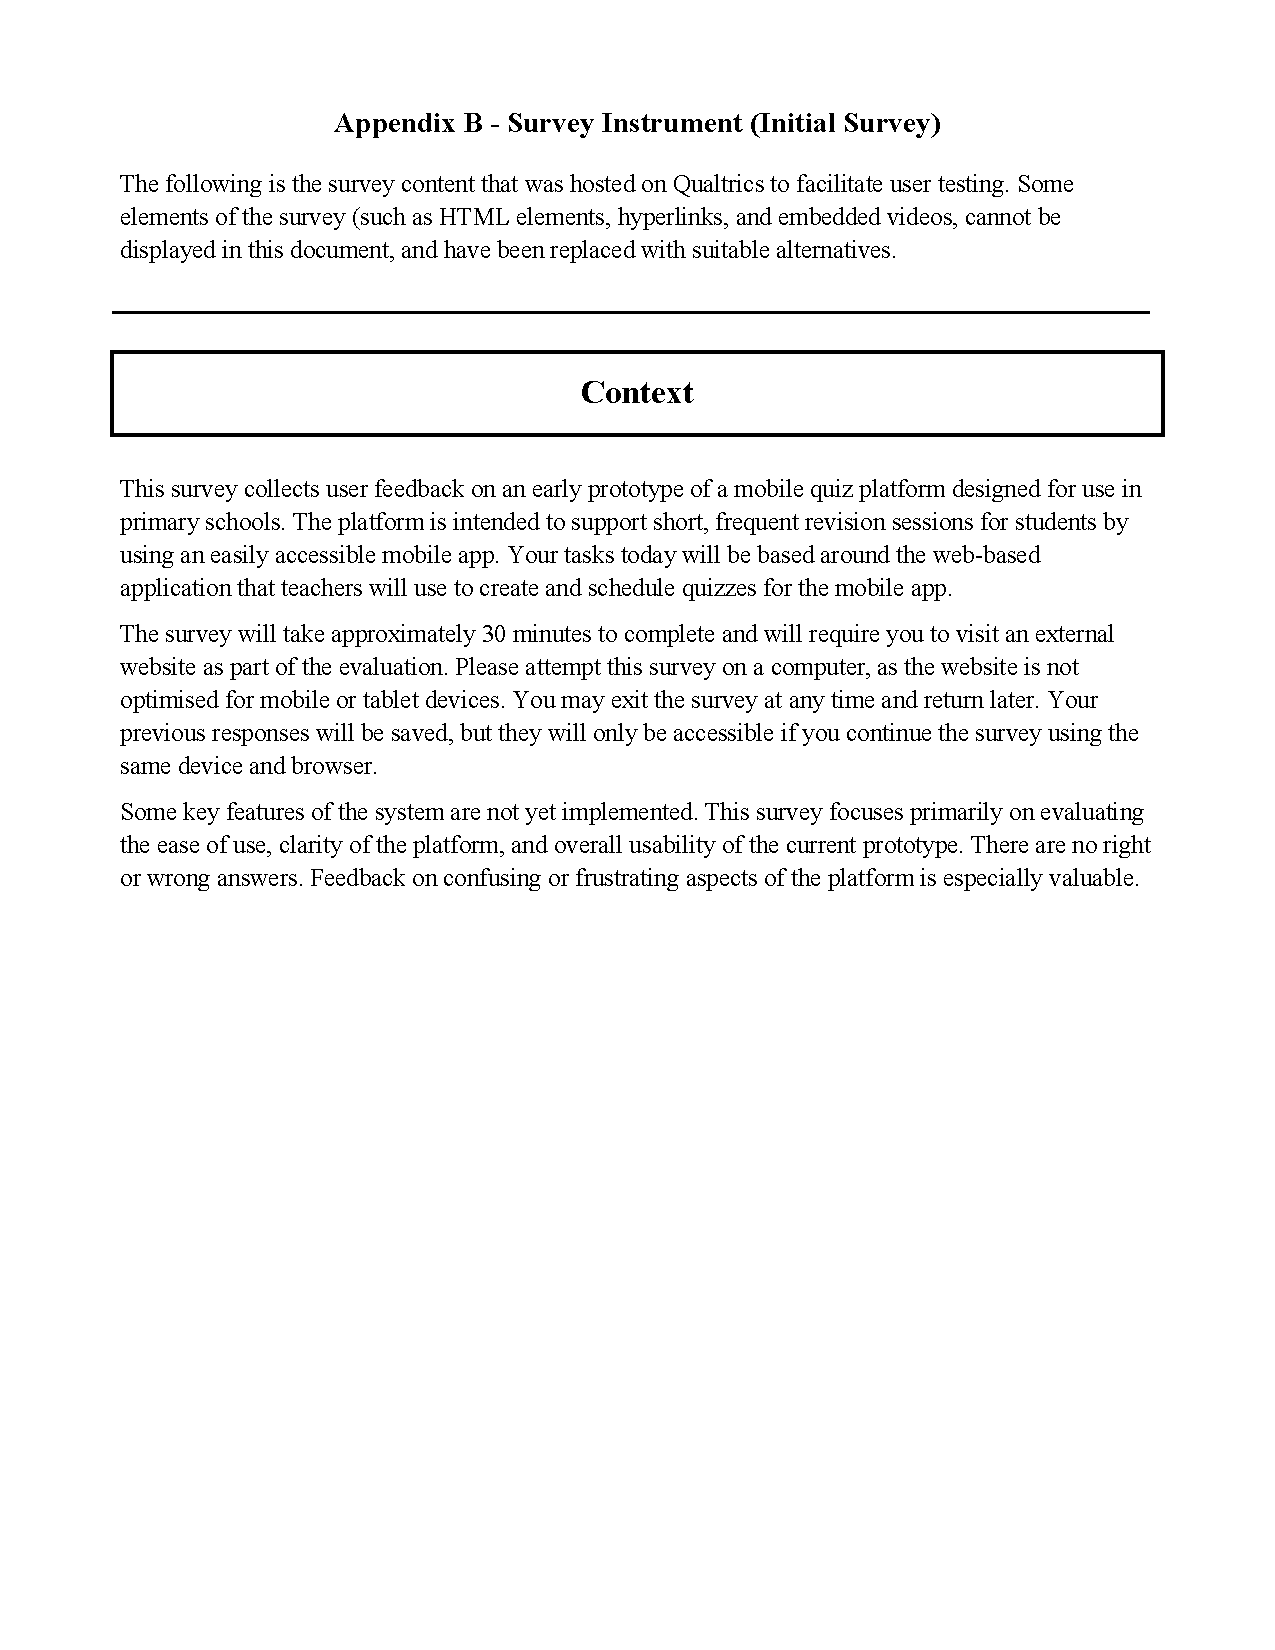
\includepdf[pages=-,pagecommand={\thispagestyle{plain}},scale=0.97]{assets/appendix-b/Figure_B_1_Survey_Instrument_Initial_Survey.pdf}

\clearpage
\phantomsection
\addcontentsline{toc}{chapter}{Appendix C - Initial User Testing Structured Results Summary}
\begin{center}
{\fontsize{14}{16}\selectfont\bfseries Appendix C - Initial User Testing Structured Results Summary\par}
\end{center}
\vspace{1cm}

\section*{1. Dataset Overview}


\begin{itemize}
\item Raw usable rows in cleaned CSV export: \textbf{11}
\item Marked as finished in CSV: \textbf{9}
\item Marked as partial in CSV: \textbf{2}
\end{itemize}

\section*{2. Method Summary}


This user testing phase mainly wanted to investigate the usability and learnability of key teacher workflows. These included the teacher dashboard functionalities of class, quiz and schedule management. The AI and gamification features were deliberately exluded in this phase, as it the main goal of this test was to gather insights on the foundational workflows before introducting the more novel features. This evaluation also wanted to find out the perceived value of the platform for teachers, as in, how well would the platform translate into real classroom use, and how likely teachers would pick up this platform in practice. To further prepare for the implementation of AI features, this evaluation also wanted to explore teachers' attitudes toward the use of AI for quiz generation, and what conditions would make them feel comfortable using such features in practice.


The main objectives of this evaluation were as follows:


\begin{enumerate}
\item Determining learnability and usability levels in relation to core teacher workflows,
\item Evaluating the clarity of quiz types and scheduling interfaces,
\item Measuring practical value and relevance of the platform for teachers, and
\item Exploring attitudes toward AI quiz generation.
\end{enumerate}

The survey was hosted on Qualtrics as it provided the flexibility to design a structured survey with complex survey flow and question types, while also allowing for the collection and visualisation of data.


The prototype platform was self-hosted and multiple teacher accounts were created beforehand to provide a smoother onboarding experience, as participants were not required to go through a tedious registration process.


Credentials were issued using a self-developed atomic credential issuer tool, which was linked to the Qualtrics survey flow. This allowed each participant to receive unique credentials for the prototype platform immediately after consenting to participate in the survey, which they could then use to log in and complete the assigned tasks on the platform.


The full survey content is provided in \textbf{Appendix B (Initial User Testing Survey Instrument)}, and the main sections of the survey were structured as scenarios. Participants were guided through four scenarios that represented common teacher-based user journeys. Each scenario had a set of associated tasks that participants were asked to complete, but step-by-step instructions were intentionally hidden to allow for a more natural first-time interaction with the platform. This allows for a better assessment of the discoverability and learnability of the platform, as well as the intuitiveness of the user interface and workflows.


The four scenarios are as follows:


\begin{enumerate}
\item \textbf{Scenario 1: Class Creation and Student Management} - This scenario focused on the process of creating a new class, adding students to the class, and managing student information.
\item \textbf{Scenario 2: Quiz Creation and Management} - This scenario focused on the process of creating quizzes, adding questions to the quiz, and managing quiz content. Tasks included creating a quiz, adding different types of questions (e.g. multiple choice, short answer), and editing quiz content. The sample quiz content that were provided to the teachers were designed to be relevant to the subjects and year groups that the teachers selected at the start of the survey, in order to make the tasks more realistic for the participants.
\item \textbf{Scenario 3: Scheduling Quizzes} - This scenario focused on the process of scheduling quizzes for students, including attempt windows, attempt limits and rescheduling flows.
\item \textbf{Scenario 4: Student Quiz Experience} - This scenario focused on the student experience of attempting a quiz and reviewing their results. No actual hands on tasks were assigned here. Teachers were just given a video walkthrough of the student quiz experience and were asked to evaluate the design and usability of the student-facing mobile application based on their observations. Gamification features were intentionally excluded from this scenario, as the main focus was on the core quiz-taking experience and the mobile interface, and not the additional engagement features.
\end{enumerate}

After each scenario, participants were given a set of Likert-scale questions to evaluate the the platform for the tasks they had just completed. These were followed by open-ended questions to gather qualitative feedback and identify specific pain points, areas of confusion, and suggestions for improvement.


Following the four scenario-based tasks, the survey included two additional sections:


\begin{enumerate}
\item Perceived value of the platform for teachers, and
\item Attitudes toward AI generation features for quizzes.
\end{enumerate}

\section*{3. Participant Background}


\subsection*{3.1 Teaching Experience}


\begin{itemize}
\item 10+: 6
\item 3-5: 3
\item 6-10: 2
\end{itemize}

\begin{center}
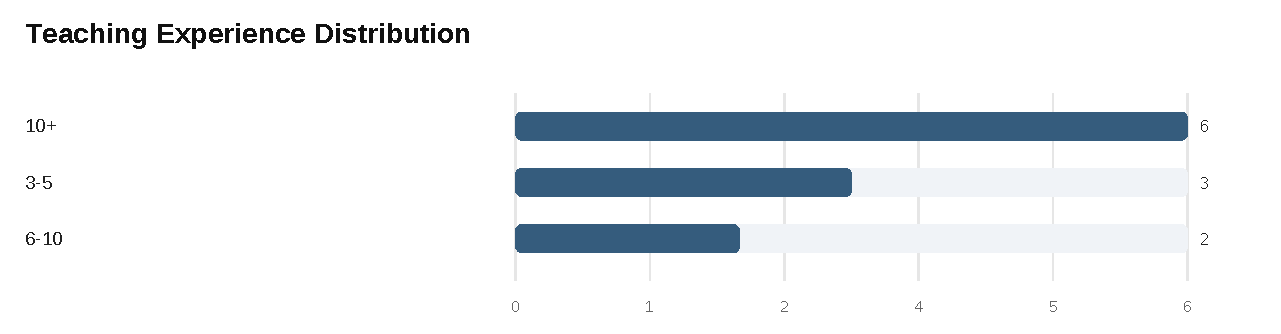
\includegraphics[width=0.94\textwidth]{assets/appendix-c/Figure_C_1_Distribution_of_Teaching_Experience_Across_the_Cleaned_Response_Set.pdf}
\end{center}


\emph{Figure C.1. Distribution of teaching experience across the cleaned response set.}


\subsection*{3.2 Frequency of Creating Revision Materials}


\begin{itemize}
\item Weekly: 8
\item Monthly: 2
\item Rarely: 1
\end{itemize}

\subsection*{3.3 Subjects Taught}


\begin{itemize}
\item Math: 7
\item English: 4
\item Science: 3
\item Mother Tongue: 1
\item PHE: 1
\end{itemize}

Some respondents selected more than one teaching subject, so these counts are not mutually exclusive.


\begin{center}
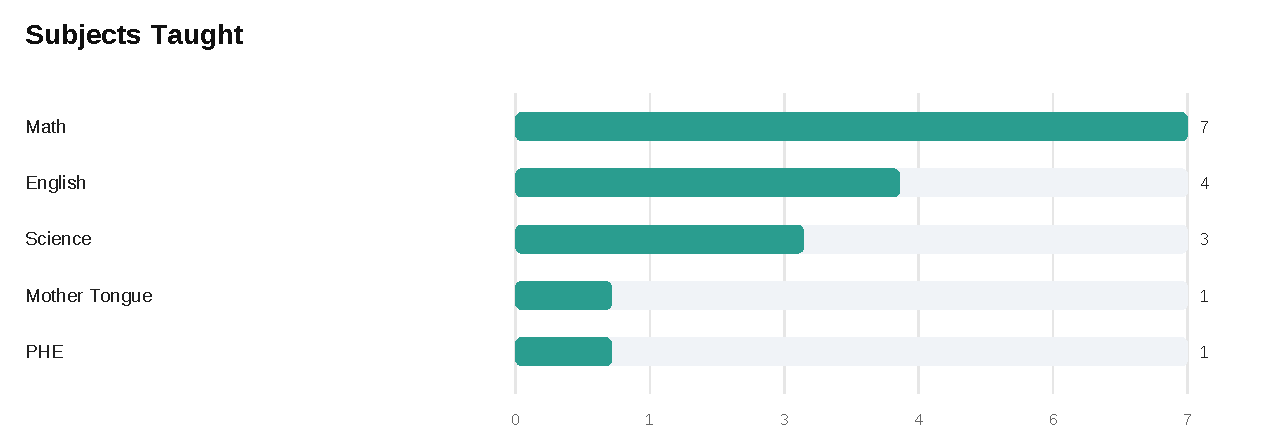
\includegraphics[width=0.94\textwidth]{assets/appendix-c/Figure_C_2_Subject_Distribution_Across_Respondents_Counts_Are_Not_Mutually_Exclusive.pdf}
\end{center}


\emph{Figure C.2. Subject distribution across respondents. Counts are not mutually exclusive.}


\section*{4. Quantitative Results by Survey Block}


\begin{center}
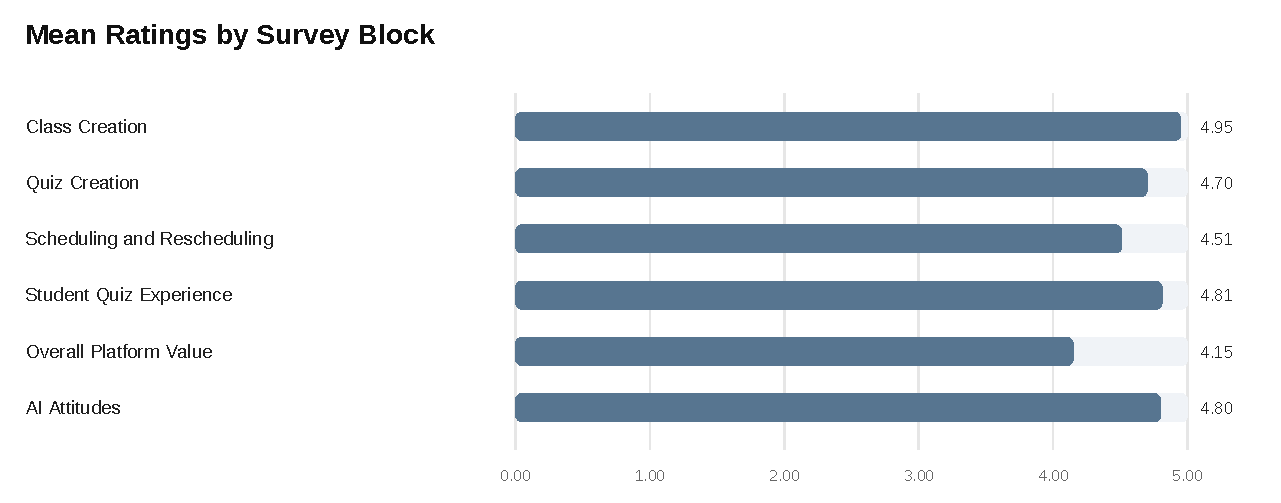
\includegraphics[width=0.94\textwidth]{assets/appendix-c/Figure_C_3_Aggregate_Mean_Score_Across_Each_Survey_Block_Based_on_the_Cleaned_CSV_Responses.pdf}
\end{center}


\emph{Figure C.3. Aggregate mean score across each survey block, based on the cleaned CSV responses.}


\subsection*{4.1 Class Creation}


\begin{itemize}
\item Respondents with data in this block: \textbf{11}
\item Aggregate mean across block: \textbf{4.95 / 5.00}
\end{itemize}

{
\fontsize{10}{12}\selectfont
\setlength{\tabcolsep}{4pt}
\renewcommand{\arraystretch}{1.15}
\begin{xltabular}{\textwidth}{|>{\raggedright\arraybackslash}X|>{\raggedleft\arraybackslash}p{0.55cm}|>{\raggedleft\arraybackslash}p{0.95cm}|>{\raggedleft\arraybackslash}p{1.55cm}|>{\raggedleft\arraybackslash}p{2.35cm}|>{\raggedleft\arraybackslash}p{1.85cm}|}
\hline
\textbf{Item} & \textbf{n} & \textbf{Mean} & \textbf{Strongly agree} & \textbf{Agree / Somewhat agree} & \textbf{Neither / Disagree} \\ \hline
\endhead
The process of creating and managing a class was easy to understand. & 11 & 4.82 & 9 & 2 & 0 \\ \hline
The class setup process was guided clearly by the interface. & 11 & 5.00 & 11 & 0 & 0 \\ \hline
The terminology used was familiar and appropriate for a school setting. & 11 & 5.00 & 11 & 0 & 0 \\ \hline
Importing student information when creating a class was a straightforward process. & 11 & 5.00 & 11 & 0 & 0 \\ \hline
The student account creation process, where usernames and passwords are shown to the teacher for dissemination, felt suitable for real classroom use. & 11 & 4.91 & 10 & 1 & 0 \\ \hline
\end{xltabular}
}


\begin{center}
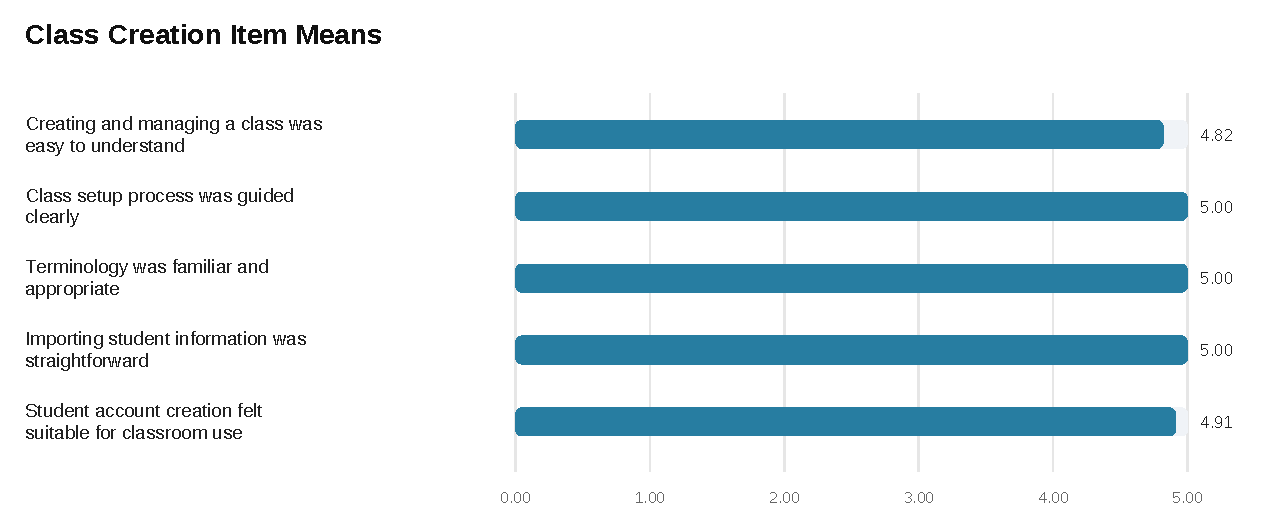
\includegraphics[width=0.94\textwidth]{assets/appendix-c/Figure_C_4_Mean_Scores_for_the_Individual_Class_Creation_Items_in_the_Initial_User_Test.pdf}
\end{center}


\emph{Figure C.4. Mean scores for the individual class-creation items in the initial user test.}


\subsection*{4.2 Quiz Creation}


\begin{itemize}
\item Respondents with data in this block: \textbf{10}
\item Aggregate mean across block: \textbf{4.70 / 5.00}
\end{itemize}

{
\fontsize{10}{12}\selectfont
\setlength{\tabcolsep}{4pt}
\renewcommand{\arraystretch}{1.15}
\begin{xltabular}{\textwidth}{|>{\raggedright\arraybackslash}X|>{\raggedleft\arraybackslash}p{0.55cm}|>{\raggedleft\arraybackslash}p{0.95cm}|>{\raggedleft\arraybackslash}p{1.55cm}|>{\raggedleft\arraybackslash}p{2.35cm}|>{\raggedleft\arraybackslash}p{1.85cm}|}
\hline
\textbf{Item} & \textbf{n} & \textbf{Mean} & \textbf{Strongly agree} & \textbf{Agree / Somewhat agree} & \textbf{Neither / Disagree} \\ \hline
\endhead
The process of creating a quiz was easy to understand on first use. & 10 & 4.60 & 6 & 4 & 0 \\ \hline
The interface guided the quiz creation process in an intuitive manner. & 10 & 4.60 & 6 & 4 & 0 \\ \hline
The interface guided me naturally through quiz creation. & 10 & 4.60 & 6 & 4 & 0 \\ \hline
The differences between Basic and Crossword quizzes were easy to understand during creation. & 10 & 4.90 & 9 & 1 & 0 \\ \hline
The system provided the right amount of configuration options for quiz creation. & 10 & 4.70 & 7 & 3 & 0 \\ \hline
Each quiz type (basic, crossword, rapid) was perceived to be clear and distinct. & 10 & 4.90 & 9 & 1 & 0 \\ \hline
The available quiz types were aligned with common classroom revision practices. & 10 & 4.70 & 7 & 3 & 0 \\ \hline
The available quiz types were sufficient for supporting typical revision needs. & 10 & 4.60 & 7 & 2 & 1 \\ \hline
\end{xltabular}
}


\begin{center}
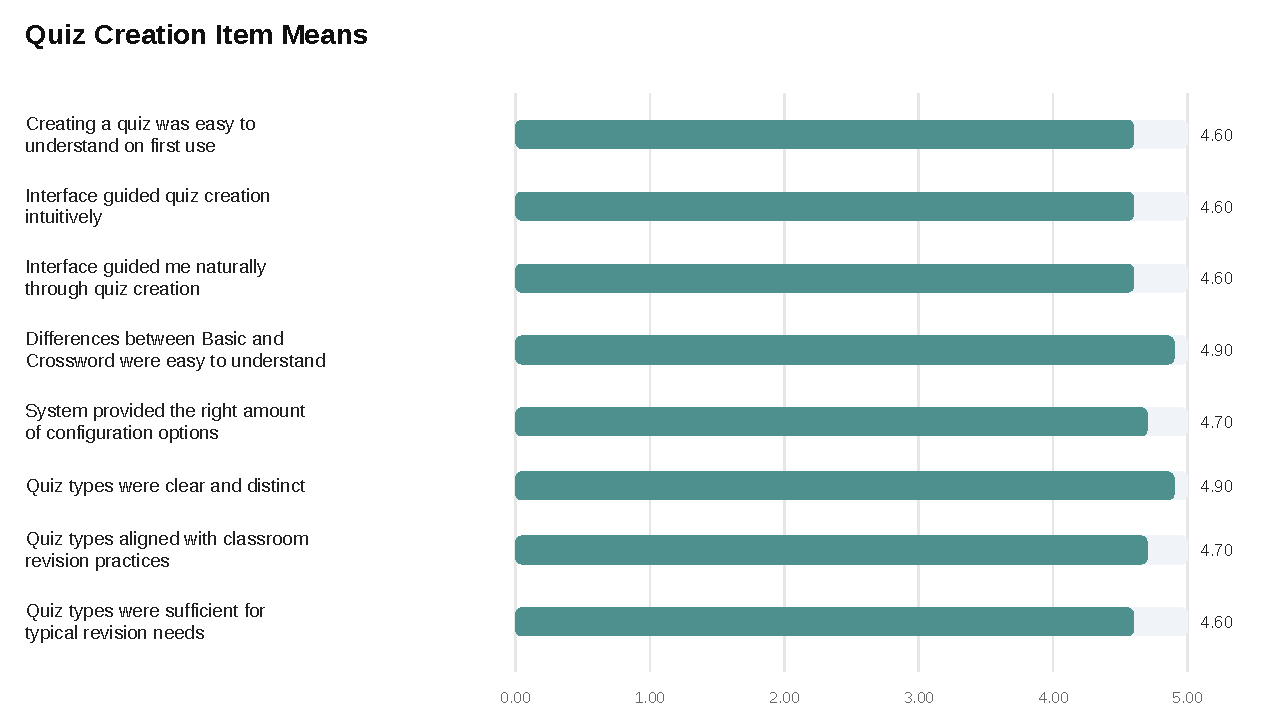
\includegraphics[width=0.94\textwidth]{assets/appendix-c/Figure_C_5_Mean_Scores_for_the_Individual_Quiz_Creation_Items_in_the_Initial_User_Test.pdf}
\end{center}


\emph{Figure C.5. Mean scores for the individual quiz-creation items in the initial user test.}


\subsection*{4.3 Scheduling and Rescheduling}


\begin{itemize}
\item Respondents with data in this block: \textbf{9}
\item Aggregate mean across block: \textbf{4.51 / 5.00}
\end{itemize}

{
\fontsize{10}{12}\selectfont
\setlength{\tabcolsep}{4pt}
\renewcommand{\arraystretch}{1.15}
\begin{xltabular}{\textwidth}{|>{\raggedright\arraybackslash}X|>{\raggedleft\arraybackslash}p{0.55cm}|>{\raggedleft\arraybackslash}p{0.95cm}|>{\raggedleft\arraybackslash}p{1.55cm}|>{\raggedleft\arraybackslash}p{2.35cm}|>{\raggedleft\arraybackslash}p{1.85cm}|}
\hline
\textbf{Item} & \textbf{n} & \textbf{Mean} & \textbf{Strongly agree} & \textbf{Agree / Somewhat agree} & \textbf{Neither / Disagree} \\ \hline
\endhead
The location for scheduling a quiz was easy to identify. & 9 & 4.33 & 7 & 0 & 2 \\ \hline
The scheduling process was easy to understand without external instructions. & 9 & 4.78 & 7 & 2 & 0 \\ \hline
The interface guided me naturally through the scheduling process. & 9 & 4.67 & 8 & 0 & 1 \\ \hline
The system provided sufficient feedback when I scheduled or moved a quiz. & 9 & 4.56 & 6 & 2 & 1 \\ \hline
Clear feedback was provided when quizzes were scheduled, moved, or updated. & 9 & 4.67 & 6 & 3 & 0 \\ \hline
It was easy to adjust or correct a scheduling mistake. & 9 & 4.33 & 5 & 3 & 1 \\ \hline
Rescheduling a quiz was straightforward. & 9 & 4.11 & 3 & 5 & 1 \\ \hline
I felt confident that my changes to the schedule were saved correctly. & 9 & 4.67 & 7 & 1 & 1 \\ \hline
\end{xltabular}
}


\begin{center}
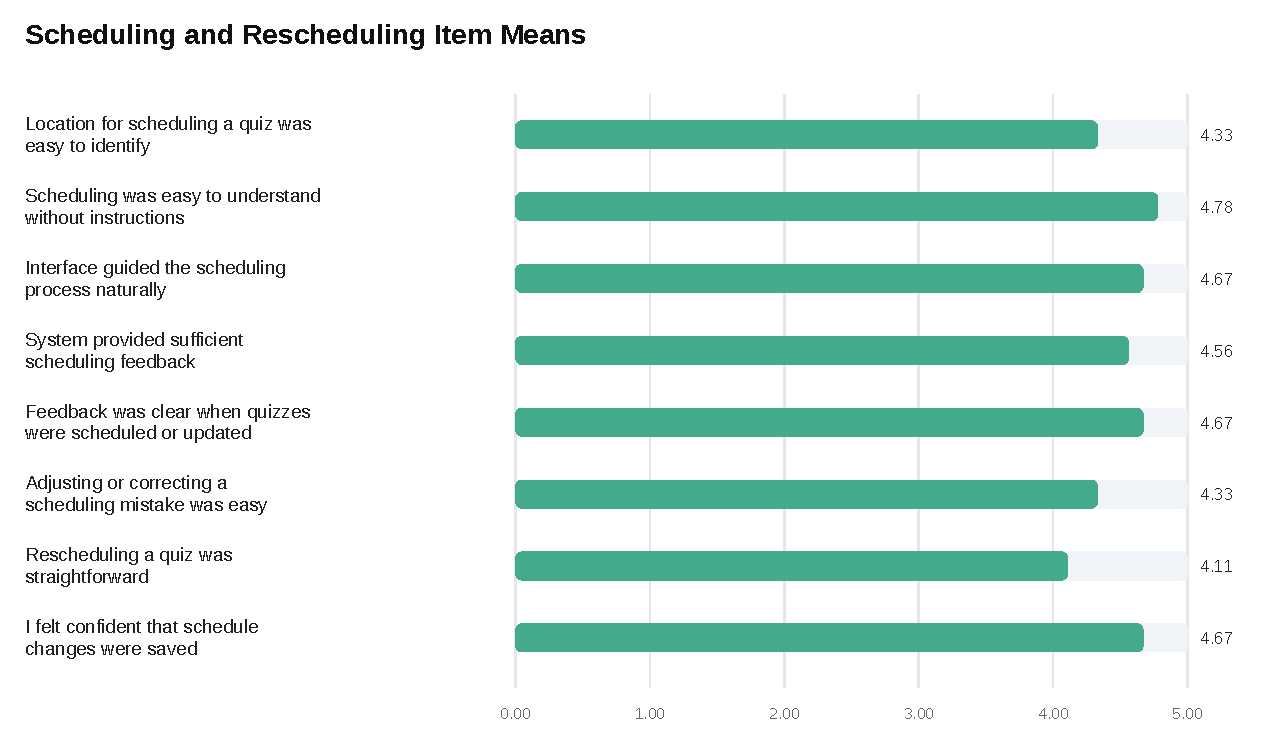
\includegraphics[width=0.94\textwidth]{assets/appendix-c/Figure_C_6_Mean_Scores_for_the_Individual_Scheduling_and_Rescheduling_Items_in_the_Initial_User_Test.pdf}
\end{center}


\emph{Figure C.6. Mean scores for the individual scheduling and rescheduling items in the initial user test.}


\subsection*{4.4 Student Quiz Experience}


\begin{itemize}
\item Respondents with data in this block: \textbf{9}
\item Aggregate mean across block: \textbf{4.81 / 5.00}
\end{itemize}

{
\fontsize{10}{12}\selectfont
\setlength{\tabcolsep}{4pt}
\renewcommand{\arraystretch}{1.15}
\begin{xltabular}{\textwidth}{|>{\raggedright\arraybackslash}X|>{\raggedleft\arraybackslash}p{0.55cm}|>{\raggedleft\arraybackslash}p{0.95cm}|>{\raggedleft\arraybackslash}p{1.55cm}|>{\raggedleft\arraybackslash}p{2.35cm}|>{\raggedleft\arraybackslash}p{1.85cm}|}
\hline
\textbf{Item} & \textbf{n} & \textbf{Mean} & \textbf{Strongly agree} & \textbf{Agree / Somewhat agree} & \textbf{Neither / Disagree} \\ \hline
\endhead
The mobile application could be used independently by students after minimal initial exposure. & 9 & 4.89 & 8 & 1 & 0 \\ \hline
The application design is well-suited for short revision sessions. & 9 & 5.00 & 9 & 0 & 0 \\ \hline
The quiz experience is engaging for students. & 9 & 4.22 & 3 & 5 & 1 \\ \hline
Time pressure during quizzes (where applicable) was perceived as appropriate rather than stressful. & 9 & 4.67 & 6 & 3 & 0 \\ \hline
A mobile application increases student accessibility to the platform, compared to a web-based platform. & 9 & 5.00 & 9 & 0 & 0 \\ \hline
Gamification features (leaderboards, scores, rewards, avatar customization) would increase student engagement. & 9 & 5.00 & 9 & 0 & 0 \\ \hline
The mobile application feels well-suited for brief, on-the-go use. & 9 & 4.89 & 8 & 1 & 0 \\ \hline
\end{xltabular}
}


\begin{center}
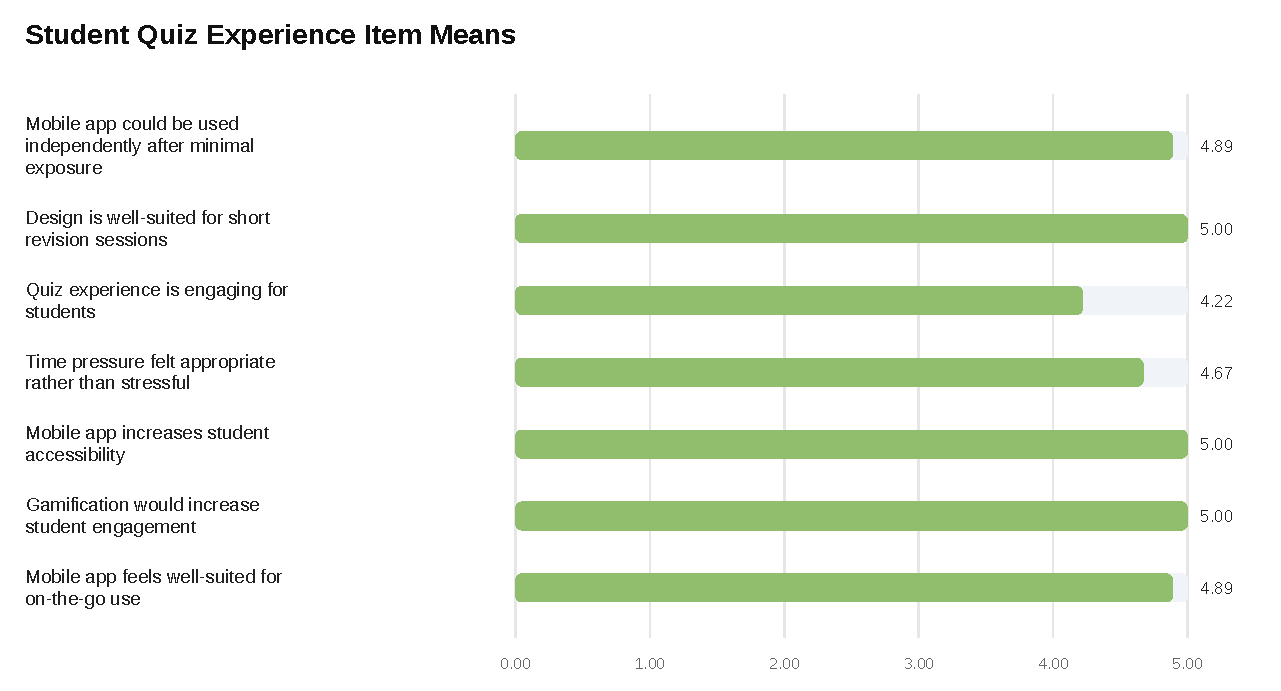
\includegraphics[width=0.94\textwidth]{assets/appendix-c/Figure_C_7_Mean_Scores_for_the_Individual_Student_Quiz_Experience_Items_in_the_Initial_User_Test.pdf}
\end{center}


\emph{Figure C.7. Mean scores for the individual student quiz experience items in the initial user test.}


\subsection*{4.5 Overall Platform Value}


\begin{itemize}
\item Respondents with data in this block: \textbf{9}
\item Aggregate mean across block: \textbf{4.15 / 5.00}
\end{itemize}

{
\fontsize{10}{12}\selectfont
\setlength{\tabcolsep}{4pt}
\renewcommand{\arraystretch}{1.15}
\begin{xltabular}{\textwidth}{|>{\raggedright\arraybackslash}X|>{\raggedleft\arraybackslash}p{0.55cm}|>{\raggedleft\arraybackslash}p{0.95cm}|>{\raggedleft\arraybackslash}p{1.55cm}|>{\raggedleft\arraybackslash}p{2.35cm}|>{\raggedleft\arraybackslash}p{1.85cm}|}
\hline
\textbf{Item} & \textbf{n} & \textbf{Mean} & \textbf{Strongly agree} & \textbf{Agree / Somewhat agree} & \textbf{Neither / Disagree} \\ \hline
\endhead
The platform feels practical for day-to-day classroom use. & 9 & 4.44 & 4 & 5 & 0 \\ \hline
The platform integrates well into my regular teaching routine. & 9 & 4.56 & 5 & 4 & 0 \\ \hline
Using this platform would save me time compared to my current revision practices. & 9 & 3.89 & 1 & 6 & 2 \\ \hline
Managing revision through this platform would feel more efficient. & 9 & 4.22 & 3 & 5 & 1 \\ \hline
The platform reduces the administrative burden of organising revision activities. & 9 & 4.11 & 3 & 4 & 2 \\ \hline
The platform provides clear value beyond my current tools. & 9 & 4.00 & 2 & 5 & 2 \\ \hline
The platform fits within typical school constraints (time, resources). & 9 & 4.00 & 1 & 7 & 1 \\ \hline
The platform encourages students to engage in independent, self-directed learning. & 9 & 4.00 & 1 & 7 & 1 \\ \hline
\end{xltabular}
}


\begin{center}
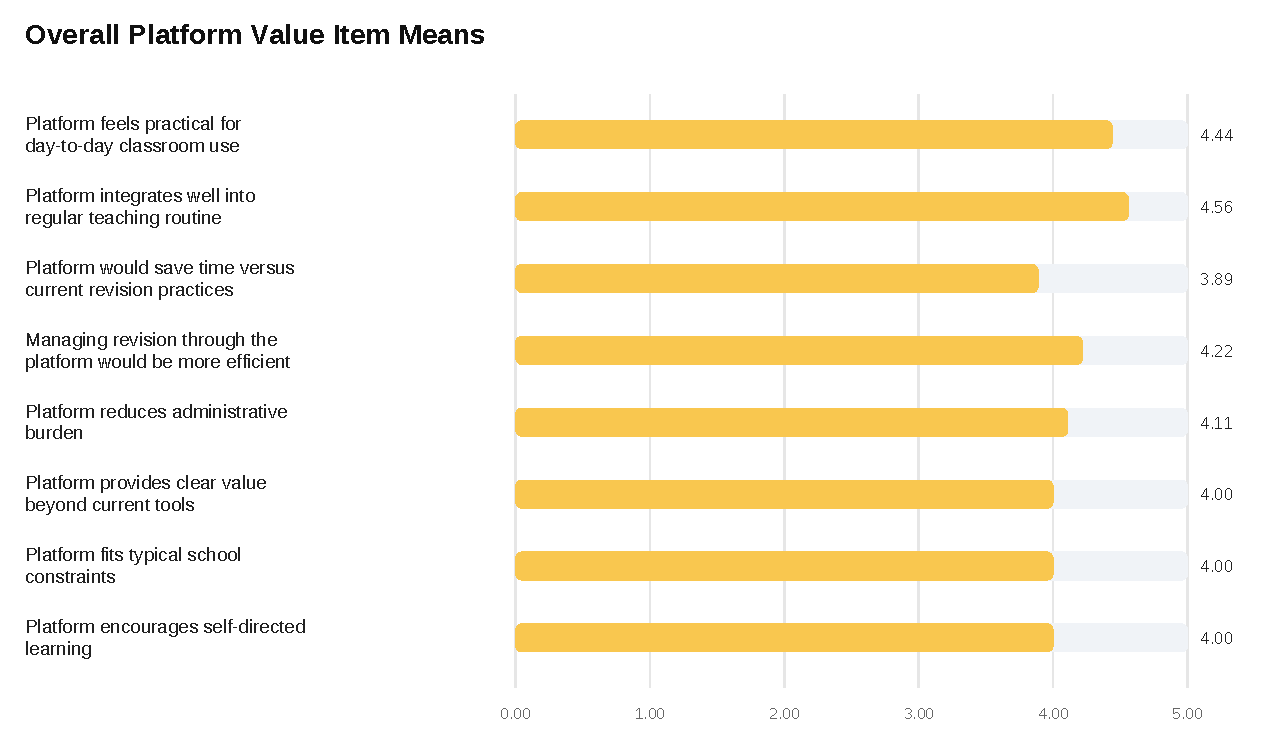
\includegraphics[width=0.94\textwidth]{assets/appendix-c/Figure_C_8_Mean_Scores_for_the_Individual_Overall_Platform_Value_Items_in_the_Initial_User_Test.pdf}
\end{center}


\emph{Figure C.8. Mean scores for the individual overall platform value items in the initial user test.}


\subsection*{4.6 AI Attitudes}


\begin{itemize}
\item Respondents with data in this block: \textbf{9}
\item Aggregate mean across block: \textbf{4.80 / 5.00}
\end{itemize}

{
\fontsize{10}{12}\selectfont
\setlength{\tabcolsep}{4pt}
\renewcommand{\arraystretch}{1.15}
\begin{xltabular}{\textwidth}{|>{\raggedright\arraybackslash}X|>{\raggedleft\arraybackslash}p{0.55cm}|>{\raggedleft\arraybackslash}p{0.95cm}|>{\raggedleft\arraybackslash}p{1.55cm}|>{\raggedleft\arraybackslash}p{2.35cm}|>{\raggedleft\arraybackslash}p{1.85cm}|}
\hline
\textbf{Item} & \textbf{n} & \textbf{Mean} & \textbf{Strongly agree} & \textbf{Agree / Somewhat agree} & \textbf{Neither / Disagree} \\ \hline
\endhead
Use of AI-generated quizzes would reduce the effort required to create revision questions. & 9 & 4.78 & 7 & 2 & 0 \\ \hline
AI-generated questions would be considered trustworthy after review. & 9 & 4.56 & 5 & 4 & 0 \\ \hline
Use of AI-generated quizzes for revision would feel comfortable and acceptable. & 9 & 4.67 & 6 & 3 & 0 \\ \hline
Control over topic coverage should be available when using AI-generated quizzes. & 9 & 5.00 & 9 & 0 & 0 \\ \hline
AI-generated quizzes should align closely with the syllabus. & 9 & 5.00 & 9 & 0 & 0 \\ \hline
\end{xltabular}
}


\begin{center}
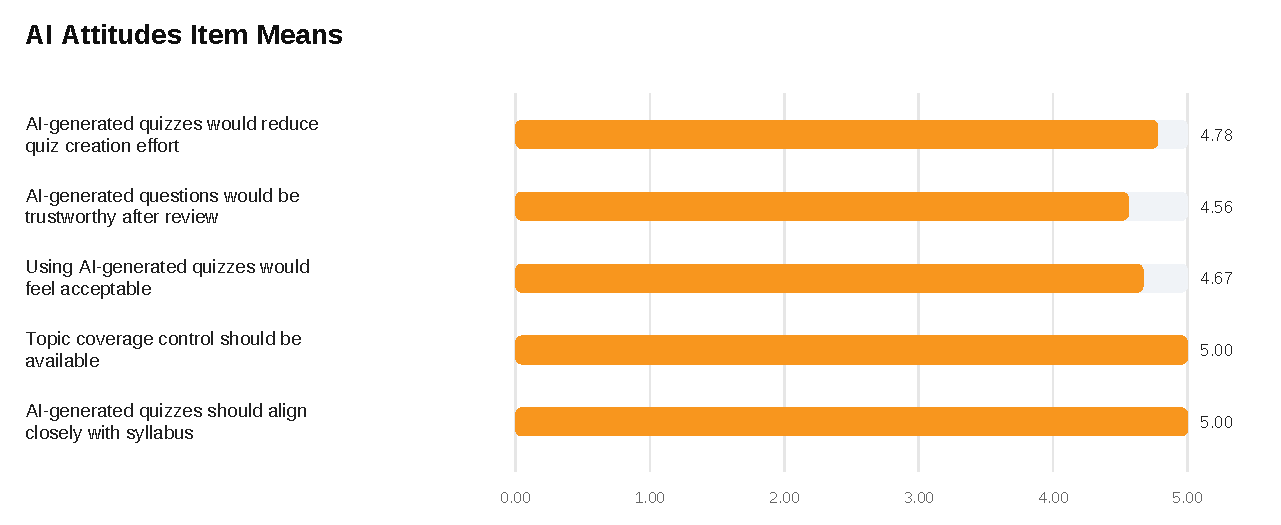
\includegraphics[width=0.94\textwidth]{assets/appendix-c/Figure_C_9_Mean_Scores_for_the_Individual_AI_Attitude_Items_in_the_Initial_User_Test.pdf}
\end{center}


\emph{Figure C.9. Mean scores for the individual AI-attitude items in the initial user test.}


\section*{5. Open-Ended Responses}


\subsection*{5.1 Class Creation}


\textbf{What parts of the class creation process felt unclear or unintuitive (if any)?}


\begin{itemize}
\item "nil"
\item "It may be useful to be able to regenerate their passwords/usernames or have a downloadable file even after the initial dissemination, in the event students forget their passwords."
\item "Some teachers might not understand what it means to save or distribute the credentials and will lose them after leaving the page. A more direct instruction to download the CSV, or making downloading the CSV a necessary step before going to the next page might be safer."
\item "Maybe a dropdown list for the level will be more user friendly."
\item "None, but the interface is not that mobile friendly."
\item "The warning about the "credentials won't be shown again". Users may still make such mistakes by not saving them despite the red font warning. Is there a function/mechanism put in place for them to still retrieve students' login credentials if such case really happens?"
\item "I think it was easy to follow since it only involves 3 steps."
\item "Do you allow teachers to create a small group teaching? So can we bypass uploading of CSV file? We want to have the option to key in students’ names directly into the system. For an e.g. i want to assign only to a differentiated group e.g. 5 students. We hope to key in the 5 names directly and form a group. A teaching class is not necessarily a full class of 35-40 students. Sometimes we just need to assign a small group to review and review certain concepts."
\end{itemize}

\subsection*{5.2 Quiz Creation}


\textbf{What parts of the quiz creation process felt unclear or unintuitive (if any)?}


\begin{itemize}
\item "Basic Quiz. "Context" option. I missed that out. Could we change that to a "Multi-Part Question" instead? So teachers can typed the context in the main question page and then we can add in part a), b), c) etc."
\item "The button to add the next question could be more obvious for the basic quiz."
\item "I am thinking the context in basic quiz be brought to the front tab instead of the last, as it usually sets the stem of the questions"
\item "For Basic, it took me a while to spot that there was an option for different item types, so I was wondering where to type the context question. But it's a first-time user issue, as once I spotted, it was intuitive for the rest of the questions."
\item "For MCQs, I couldn't set the next question without having to click the additional item on the left. I didn't I have to add the items to 3 before setting the 3 questions."
\item "-"
\item "1. Under "Basic" quiz type, when creating a new question by clicking "+", a new question card appears at the same spot and covered the previously created question. This transition does not visibly cue the user the end of the previous action and the beginning of a new action. A more intuitive transition could be, for example, the previous question retracts into a smaller card and moves up, then the new question card appears below when the page also moves to help user focus on the new question card. 2. Timer: when the timer toggle is off, the wording "No limit" is displayed on the right hand side of the toggle, which might mislead the user to think this toggle functions to turn on the "No limit" setting. But user will only realise the toggle is just to turn on or off the timer after clicking it and the wording changes to "On". So instead of put the wording "No limit" there, I feel just put words "On" and "Off" will be more intuitive, because the toggle shows grey colour when it is off, and green colour when turned on, which matches the common product design practice. If really need to add "No limit", maybe can put as "Off (no limit)"? 3. When creating "subject" and "topic", for first time users, there is no subject or topic in the drop down list. The option to "Select A Subject" or "Select A Topic" might be misleading the user to think by clicking the box, which looks more like a button than the "Add new..." because of the shape and colour that's one shade darker than the background drop down menu, they can choose from a list of subjects and topics. However, after creating the first subject/topic, then I realised the subject/topic label I just created will be added below for me to choose from next time when I create a quiz. Perhaps can consider not showing the "Select A Subject" or "Select A Topic" wording when there is no subject/topic created yet. So that user will see only one fuction to "Add new...+" (can consider to make the "Add new...+" to look more like a button too). The "Select A Subject" or "Select A Topic" can be shown after the first subject/topic has been created by the user as it will make more sense after there is something for users to choose from."
\end{itemize}

\textbf{What features would make quiz creation more efficient?}


\begin{itemize}
\item "If the add question button stays on top even as questions are being added."
\item "See above."
\item "For the crossword quiz, it can be placed at the bottom right corner so that users do not need to scroll up all the way to add a new word."
\item "By uploading a quiz in word document or pdf file and it automatically churns out"
\item "Just a cosmetic issue... I was uncomfortable with the size and position of the box for the question text. It felt too small and the position of it on the left of the options felt 'weird'. I think most teachers are used to seeing the question being above the options."
\item "If can do away with that and just keep the "next question" button when needing to create more questions would make it easier."
\item "It will be great if there’s an AI function to generate similar questions while keeping the question stem identical (extra practice for math)"
\item "AI generated questions and answers. Users could just enter subject and topic as prompt for the AI to generate questions then user can edit based on that."
\item "You can provide question banks for the three main types of learning progress e.g. Low progress, Middle progress and High progress."
\end{itemize}

\textbf{Are there any types of revision activities you commonly use that are not well supported by the current quiz types?}


\begin{itemize}
\item "-"
\item "The option for students to submit a drawing. Teachers can upload a background template and students can annotate or draw on it during submission."
\item "Flash card, True / False, any spot the difference games :X ?"
\item "Not so much the revision activity, but the feedback that can be provided to the student after they attempt the questions."
\item "The type with check boxes. Check all boxes that are correct."
\item "Prompts/hints given to students when they attempted the question incorrectly for them to reattempt the questions"
\item "Not any at the moment."
\item "Currently, we are using SLS and they can assign quizzes to a small group of students, not necessarily a full class"
\end{itemize}

\subsection*{5.3 Scheduling and Rescheduling}


\textbf{What parts of the scheduling process felt unclear or unintuitive (if any)?}


\begin{itemize}
\item "Tendency to go back to the quiz and click on the edit button."
\item "nil"
\item "There was no button to click on to reschedule. It took a few tries to figure out that it was a right-click on the calendar. It would be useful to have an option to see all the quizzes assigned and edit the schedule from there."
\item "I did not watch the video but I trial and error and did a right click to edit the schedule. I got it by chance. (screen interface) I need to decrease the screen size to 90\%, then I am able to click the assign tab."
\item "Again, first-time user issue. Didn't see the instructions to right-click to edit at first. Also, when scheduling the quiz, the pop-out with the editing selections is cut off when the page zoom was at 100\%. I could only see the 'schedule' button at the bottom when zoomed out to 80\%. Not all teachers may be savvy enough to know how to zoom out. Could that pop-out have a scroll so that the bottom can be seen regardless of zoom setting?"
\item "I wasn't sure the scheduling of quzzies is done under "Quzzies" or "class". After changing the dates and other details of the quzzies, I wasn't sure how to get out of it and go back to the page."
\item "I couldn’t do it via phone. The interface doesn’t quite support the use of Iphone"
\item "Even though there is a prompt on the hovering card saying "right click to edit details", it took me some time to figure out I need to right click the quiz "bar" to edit the details. Perhaps the prompt can indicate more specifically where to right click?"
\end{itemize}

\textbf{Are there any real classroom or school constraints that might make scheduling quizzes difficult using this system?}


\begin{itemize}
\item "nil"
\item "nil"
\item "What would happen if the student already attempted the quiz 3 times before I edit to 2 attempts only? Would the results still be saved?"
\item "-"
\item "Nil"
\item "I couldn’t find the reschedule button on the right"
\item "Not any."
\end{itemize}

\subsection*{5.4 Student Quiz Experience}


\textbf{What parts of the student quiz experience might confuse a primary school student?}


\begin{itemize}
\item "nil"
\item "a"
\item "nil"
\item "For the context item, the students may prefer having a pop-up to refer to the context while completing the following questions, instead of having to click back."
\item "-"
\item "None I can think of at the moment"
\item "I think it is user friendly enough, even for primary school students."
\item "Will there be notifications for them to access the platform when teachers schedule a quiz?"
\item "Not any"
\end{itemize}

\textbf{What factors might prevent students from using this application regularly in practice?}


\begin{itemize}
\item "parental permission to use device"
\item "a"
\item "To make the students' interface more kids friendly? add in more colours, font type can be more kids friendly, don't keep it to black"
\item "Gamification can be included or more animation for getting the answers correct or wrong."
\item "May provide Interactive goal/game features eg. one group competing to win another group to solve questions to meet a goal ..."
\item "Not sure how much data this might use... there might be parents who are on a limited budget and may not like their children constantly using up the data."
\item "All words and very few diagrams."
\item "Accessibility to mobile devices, motivation to learn via this platform"
\item "No access to phones/devices if parents do not allow."
\end{itemize}

\subsection*{5.5 Other Feedback}


\textbf{Any other feedback?}


\begin{itemize}
\item "nil"
\item "Perhaps can have an option for teachers to upload the questions by uploading pdf/csv files? So teachers don't have to type in questions one by one but upload the questions all at once."
\item "It is a straightforward platform for teachers to use for daily revision, but there are many platforms that provide the same experience. However, I do like that the interface is suitable on a mobile device so even if the students do not have access to computers at home, they can simply use a mobile phone to complete the quizzes. Thank you for thinking of teachers when you created this platform!"
\item "Add in the element of fun and interactive, eg Blooket game features"
\item "Nil"
\item "Nil, thanks for making the interface user friendly and lag-free"
\item "Not any"
\end{itemize}


\clearpage
\phantomsection
\addcontentsline{toc}{chapter}{Appendix D - Survey Instrument (Follow Up Survey)}

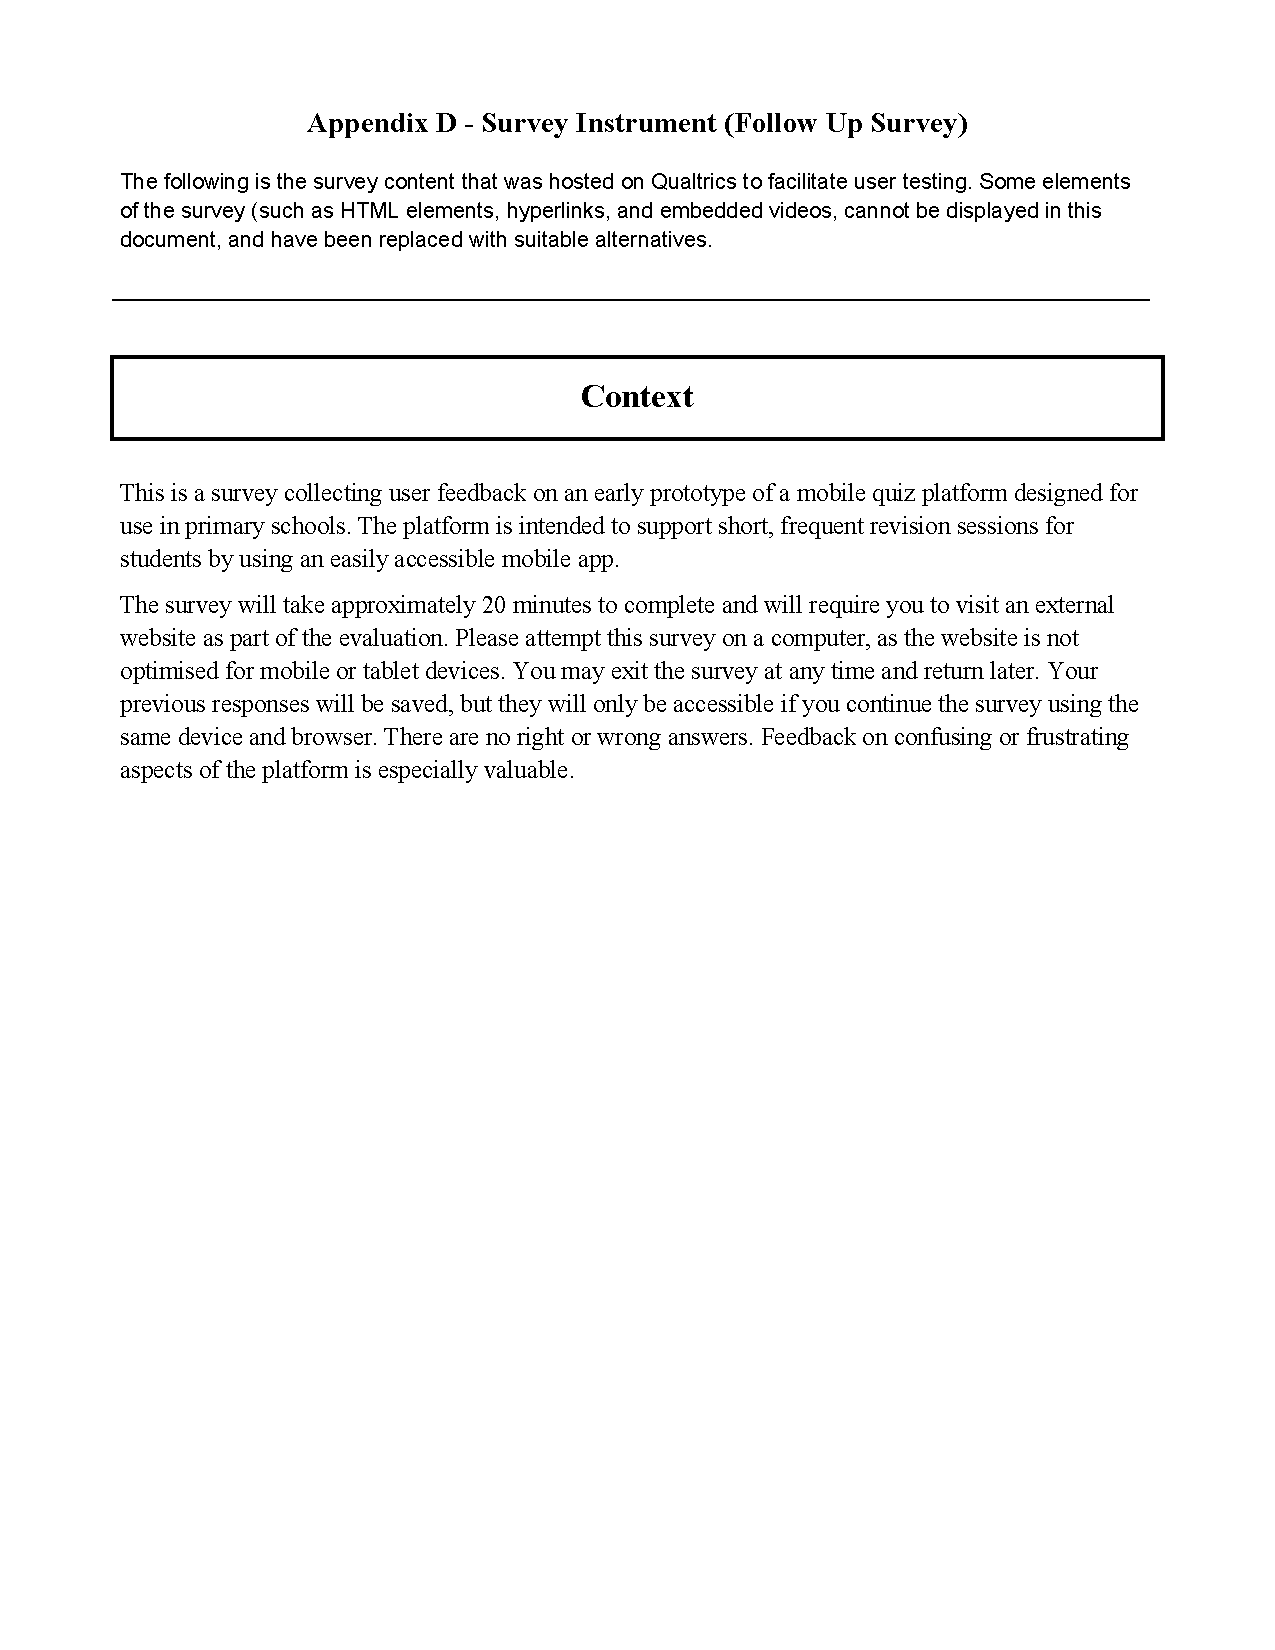
\includepdf[pages=-,pagecommand={\thispagestyle{plain}},scale=0.97]{assets/appendix-d/Figure_D_1_Survey_Instrument_Follow_Up_Survey.pdf}

\clearpage
\phantomsection
\addcontentsline{toc}{chapter}{Appendix E - Follow Up User Testing Structured Results Summary}
\begin{center}
{\fontsize{14}{16}\selectfont\bfseries Appendix E - Follow Up User Testing Structured Results Summary\par}
\end{center}
\vspace{1cm}

\section*{1. Dataset Overview}


\begin{itemize}
\item Raw usable rows in export: \textbf{9}
\item Marked as finished in CSV: \textbf{9}
\item Marked as partial in CSV: \textbf{0}
\item Mean completion time: \textbf{1,727 seconds} (approximately \textbf{28.8 minutes})
\end{itemize}

\section*{2. Method Summary}


Since the last phase, the scheduling interface was redesigned to be more intuitive. Previously, scheduling was treated as a secondary function, hidden within the quiz interface and class interface. Furthermore, rescheduling of quizzes could only be done through the class-specific page, and if a quiz was scheduled for multiple classes, the user would have to go to each individual class page to reschedule. The previous survey also indicated discoverability problems, as teachers reported that they did not know where to find the scheduling interface. As such, the iterations made since the last phase promoted scheduling to a top-level function with a dedicated tab, accessible through the sidebar. The scheduling interface now allows for management of schedules across all classes on a single page. It also allows the easy scheduling of quizzes to multiple classes at once.


The AI generation and gamification features had also been fully implemented, and this secondary testing therefore sought to evaluate the usability of these features, as well as get a sense of teacher opinions on the quality of the generated content.


The main objectives of this secondary testing phase are therefore as follows:


\begin{enumerate}
\item Evaluating the new scheduling interface and interactions, especially for rescheduling tasks.
\item Assessing the usability of the AI generation features, as well as the quality of the generated content.
\item Gathering teacher feedback on the student app experience after the inclusion of gamification features, and evaluating the impact of gamification on the student experience.
\end{enumerate}

The survey was once again hosted on Qualtrics, and the prototype platform was self-hosted with pre-created teacher accounts to provide a smooth onboarding experience for participants. The setup was functionally the same as the first phase, but with the prototype platform updated to include the new scheduling interface, as well as the AI generation and gamification features.


The full survey content is provided in \textbf{Appendix D (Follow Up User Testing Survey Instrument)}. The survey content was structured similarly to the first phase, with scenario-based sections followed by Likert-scale and open-ended questions.


The following are the three scenarios that were included in this secondary testing phase:


\begin{enumerate}
\item \textbf{Scenario 1: Scheduling and Rescheduling Quizzes} - The exact same scheduling and rescheduling tasks from the first phase were included in this scenario. The purpose was to evaluate whether the new scheduling interface had improved the usability and discoverability of scheduling features, especially for rescheduling tasks.
\item \textbf{Scenario 2: AI Generation of Quiz Content} - This scenario asked teachers to generate quiz content using the AI generation features. Teachers were given the freedom to generate any quiz content they wanted with some constraints on the settings. They were then asked to evaluate the quality of the generated content and provide feedback on the usability of the AI generation features.
\item \textbf{Scenario 3: Student App Experience with Gamification} - This scenario showed a video walkthrough of the student app experience after the inclusion of gamification features. Teachers were then asked to evaluate the student experience and provide feedback on the impact of gamification on student engagement and motivation.
\end{enumerate}

Each scenario was followed by a set of Likert-scale questions and open-ended questions to gather quantitative and qualitative feedback.


\section*{3. Participant Background}


\subsection*{3.1 Teaching Experience}


\begin{itemize}
\item \texttt{10+}: 4
\item \texttt{6-10}: 3
\item \texttt{3-5}: 2
\end{itemize}

\subsection*{3.2 Teaching Levels}


\begin{itemize}
\item \texttt{Primary 6}: 7
\item \texttt{Primary 5}: 4
\item \texttt{Primary 4}: 3
\item \texttt{Primary 3}: 1
\item \texttt{Primary 1}: 1
\end{itemize}

Some respondents selected more than one teaching level, so these counts are not mutually exclusive.


\subsection*{3.3 Subjects Taught}


\begin{itemize}
\item \texttt{Math}: 6
\item \texttt{Science}: 4
\item \texttt{English}: 3
\item \texttt{Other}: 1
\end{itemize}

Some respondents selected more than one teaching subject, so these counts are not mutually exclusive.


\section*{4. Quantitative Results by Survey Block}


\subsection*{4.1 Scheduling and Rescheduling}


\begin{itemize}
\item Respondents with data in this block: \textbf{9}
\item Aggregate mean across block: \textbf{4.63 / 5.00}
\end{itemize}

{
\fontsize{10}{12}\selectfont
\setlength{\tabcolsep}{4pt}
\renewcommand{\arraystretch}{1.15}
\begin{xltabular}{\textwidth}{|>{\raggedright\arraybackslash}X|>{\raggedleft\arraybackslash}p{0.55cm}|>{\raggedleft\arraybackslash}p{0.95cm}|>{\raggedleft\arraybackslash}p{1.55cm}|>{\raggedleft\arraybackslash}p{2.35cm}|>{\raggedleft\arraybackslash}p{1.85cm}|}
\hline
\textbf{Item} & \textbf{n} & \textbf{Mean} & \textbf{Strongly agree} & \textbf{Agree / Somewhat agree} & \textbf{Neither / Disagree} \\ \hline
\endhead
The location for scheduling a quiz was easy to identify. & 9 & 5.00 & 9 & 0 & 0 \\ \hline
The scheduling process was easy to understand without external instructions. & 9 & 4.78 & 7 & 2 & 0 \\ \hline
The interface guided me naturally through the scheduling process. & 9 & 4.89 & 8 & 1 & 0 \\ \hline
Clear feedback was provided when quizzes were scheduled, moved, or updated. & 9 & 4.33 & 6 & 2 & 1 \\ \hline
It was easy to adjust or correct a scheduling mistake. & 9 & 4.44 & 7 & 1 & 1 \\ \hline
Rescheduling a quiz was straightforward. & 9 & 4.44 & 7 & 1 & 1 \\ \hline
I felt confident that my changes to the schedule were saved correctly. & 9 & 4.56 & 8 & 0 & 1 \\ \hline
\end{xltabular}
}


\begin{center}
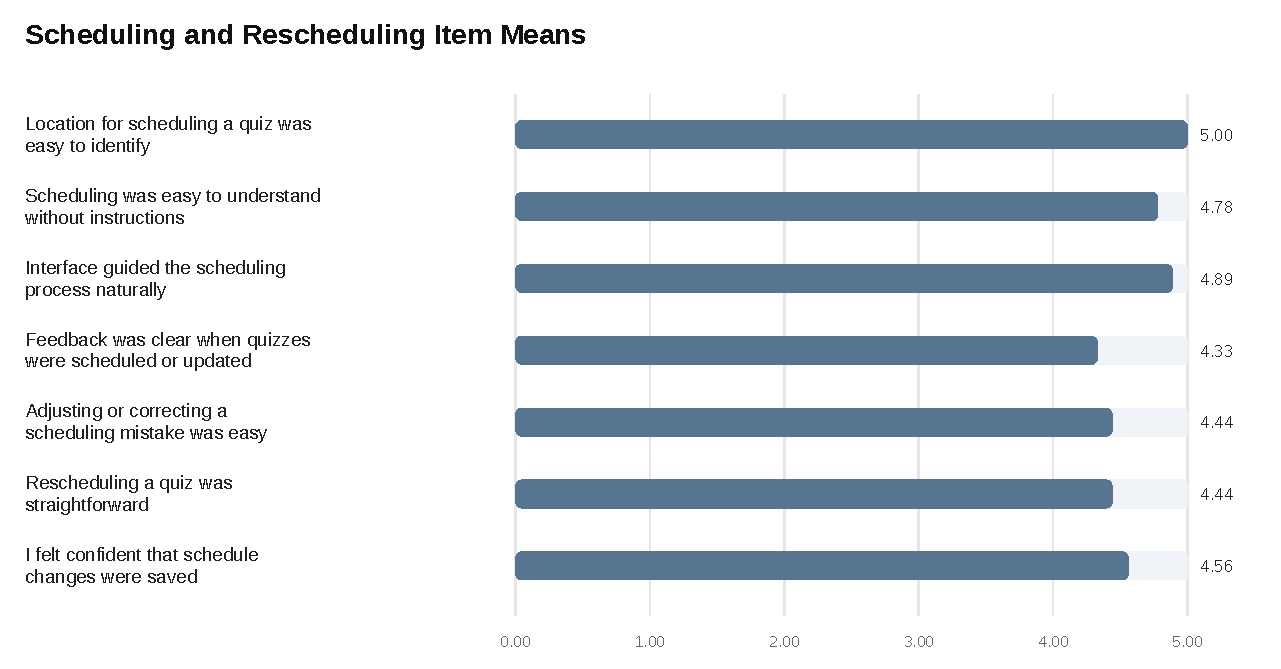
\includegraphics[width=0.94\textwidth]{assets/appendix-e/Figure_E_1_Mean_Scores_for_the_Individual_Scheduling_and_Rescheduling_Items_in_the_Follow_Up_User_Test.pdf}
\end{center}


\emph{Figure E.1. Mean scores for the individual scheduling and rescheduling items in the follow-up user test.}


\subsection*{4.2 AI Quiz Generation Interface}


\begin{itemize}
\item Aggregate mean across block: \textbf{4.85 / 5.00}
\end{itemize}

{
\fontsize{10}{12}\selectfont
\setlength{\tabcolsep}{4pt}
\renewcommand{\arraystretch}{1.15}
\begin{xltabular}{\textwidth}{|>{\raggedright\arraybackslash}X|>{\raggedleft\arraybackslash}p{0.55cm}|>{\raggedleft\arraybackslash}p{0.95cm}|>{\raggedleft\arraybackslash}p{1.55cm}|>{\raggedleft\arraybackslash}p{2.35cm}|>{\raggedleft\arraybackslash}p{1.85cm}|}
\hline
\textbf{Item} & \textbf{n} & \textbf{Mean} & \textbf{Strongly agree} & \textbf{Agree / Somewhat agree} & \textbf{Neither / Disagree} \\ \hline
\endhead
The location of the AI quiz generation feature was easy to identify. & 9 & 4.89 & 8 & 1 & 0 \\ \hline
The AI generation interface was easy to understand without external instructions. & 9 & 4.89 & 8 & 1 & 0 \\ \hline
The available generation settings (subject, level, instructions, etc.) were clearly presented. & 9 & 4.78 & 7 & 2 & 0 \\ \hline
It was easy to configure the settings needed to generate a quiz. & 9 & 4.89 & 8 & 1 & 0 \\ \hline
The process of generating quizzes using the AI tool was straightforward. & 9 & 4.78 & 7 & 2 & 0 \\ \hline
The system clearly indicated when quiz generation was in progress or successful. & 9 & 4.89 & 8 & 1 & 0 \\ \hline
\end{xltabular}
}


\begin{center}
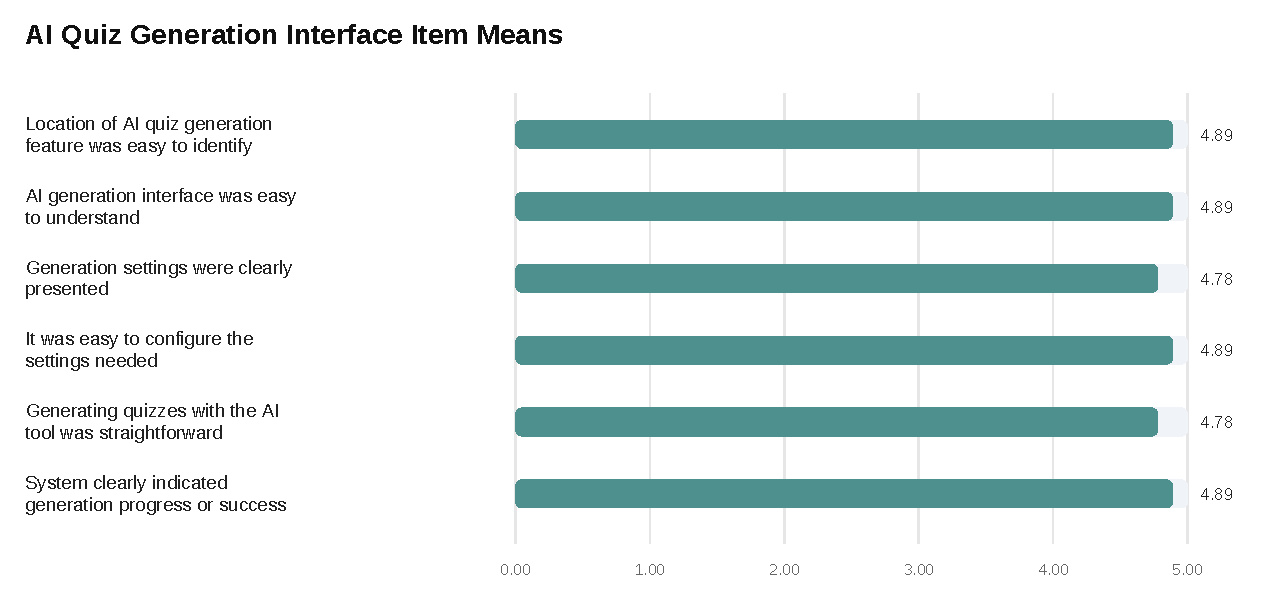
\includegraphics[width=0.94\textwidth]{assets/appendix-e/Figure_E_2_Mean_Scores_for_the_Individual_AI_Quiz_Generation_Interface_Items_in_the_Follow_Up_User_Test.pdf}
\end{center}


\emph{Figure E.2. Mean scores for the individual AI quiz generation interface items in the follow-up user test.}


\subsection*{4.3 AI Generated Output}


\begin{itemize}
\item Aggregate mean across block: \textbf{4.40 / 5.00}
\end{itemize}

{
\fontsize{10}{12}\selectfont
\setlength{\tabcolsep}{4pt}
\renewcommand{\arraystretch}{1.15}
\begin{xltabular}{\textwidth}{|>{\raggedright\arraybackslash}X|>{\raggedleft\arraybackslash}p{0.55cm}|>{\raggedleft\arraybackslash}p{0.95cm}|>{\raggedleft\arraybackslash}p{1.55cm}|>{\raggedleft\arraybackslash}p{2.35cm}|>{\raggedleft\arraybackslash}p{1.85cm}|}
\hline
\textbf{Item} & \textbf{n} & \textbf{Mean} & \textbf{Strongly agree} & \textbf{Agree / Somewhat agree} & \textbf{Neither / Disagree} \\ \hline
\endhead
The generated quizzes followed the topic or instructions that I provided. & 9 & 4.56 & 5 & 4 & 0 \\ \hline
The difficulty level of the generated questions was appropriate for the selected education level. & 9 & 4.11 & 3 & 5 & 1 \\ \hline
The generated questions appeared factually correct. & 9 & 4.56 & 5 & 4 & 0 \\ \hline
The answer options and correct answers were unambiguous. & 9 & 4.33 & 3 & 6 & 0 \\ \hline
The questions did not feel repetitive. & 9 & 4.44 & 4 & 5 & 0 \\ \hline
\end{xltabular}
}


\begin{center}
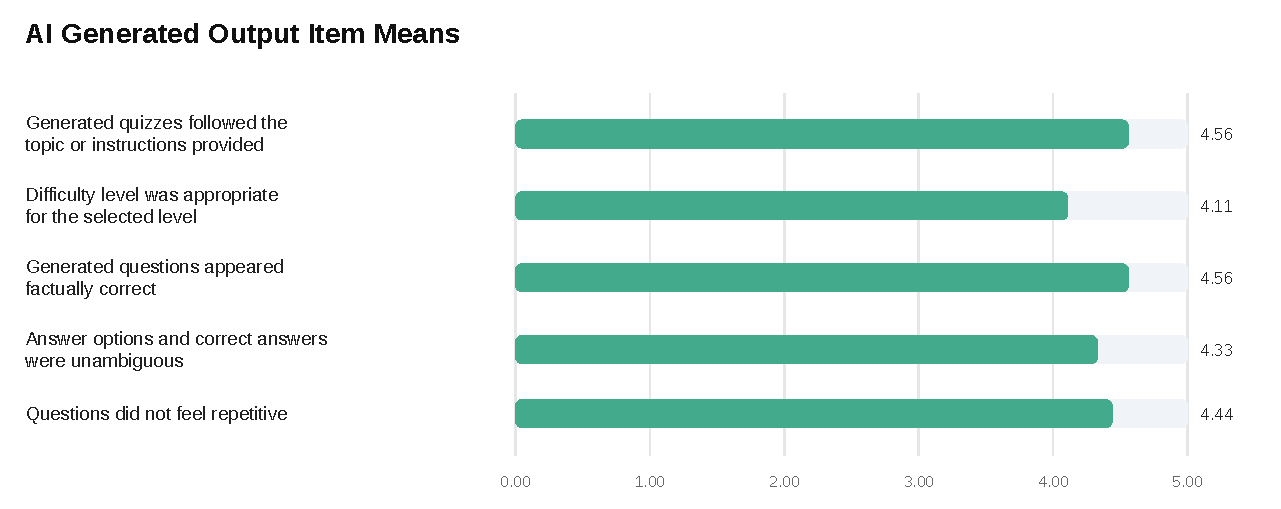
\includegraphics[width=0.94\textwidth]{assets/appendix-e/Figure_E_3_Mean_Scores_for_the_Individual_AI_Generated_Output_Items_in_the_Follow_Up_User_Test.pdf}
\end{center}


\emph{Figure E.3. Mean scores for the individual AI-generated output items in the follow-up user test.}


\subsection*{4.4 Gamification Review}


\begin{itemize}
\item Aggregate mean across block: \textbf{4.67 / 5.00}
\end{itemize}

{
\fontsize{10}{12}\selectfont
\setlength{\tabcolsep}{4pt}
\renewcommand{\arraystretch}{1.15}
\begin{xltabular}{\textwidth}{|>{\raggedright\arraybackslash}X|>{\raggedleft\arraybackslash}p{0.55cm}|>{\raggedleft\arraybackslash}p{0.95cm}|>{\raggedleft\arraybackslash}p{1.55cm}|>{\raggedleft\arraybackslash}p{2.35cm}|>{\raggedleft\arraybackslash}p{1.85cm}|}
\hline
\textbf{Item} & \textbf{n} & \textbf{Mean} & \textbf{Strongly agree} & \textbf{Agree / Somewhat agree} & \textbf{Neither / Disagree} \\ \hline
\endhead
The avatar customisation system would motivate students to participate more consistently. & 9 & 4.44 & 4 & 5 & 0 \\ \hline
The leaderboard system would encourage students to participate more consistently. & 9 & 4.78 & 7 & 2 & 0 \\ \hline
The badge system would motivate students to participate more consistently. & 9 & 4.56 & 5 & 4 & 0 \\ \hline
Overall, the reward systems shown would make quiz practice more engaging for students. & 9 & 4.67 & 6 & 3 & 0 \\ \hline
The gamification elements shown are appropriate for primary school students. & 9 & 4.78 & 7 & 2 & 0 \\ \hline
The competitive elements (leaderboards) are suitable for a classroom environment. & 9 & 4.78 & 7 & 2 & 0 \\ \hline
\end{xltabular}
}


\begin{center}
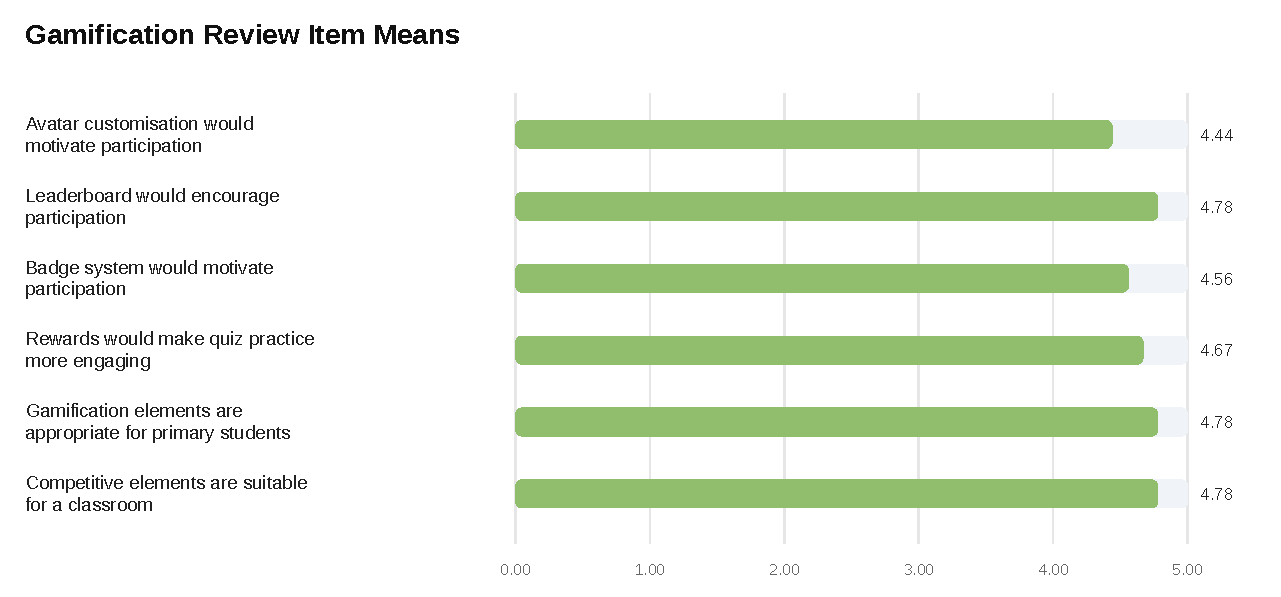
\includegraphics[width=0.94\textwidth]{assets/appendix-e/Figure_E_4_Mean_Scores_for_the_Individual_Gamification_Review_Items_in_the_Follow_Up_User_Test.pdf}
\end{center}


\emph{Figure E.4. Mean scores for the individual gamification-review items in the follow-up user test.}


\section*{5. Open-Ended Responses}


\subsection*{5.1 Scheduling and Rescheduling}


\textbf{What parts of the scheduling process felt unclear or unintuitive (if any)?}


\begin{itemize}
\item nil
\item Initial instinct when attempting to edit a scheduled quiz was to left click on the quiz instead of right click.
\item i was stuck at the scheduling pop out box. after filling up all the info, the process was stopped with no buttons to submit etc. Maybe at the scheduling page, the selection of the quizzes can add the check box on the left.
\item NIL, all parts were quite clear and guided.
\item Not sure if it was just my computer, but the 'schedule' button to click when scheduling a quiz cannot be seen when the browser zoom was at 100\%. I needed to zoom out to 80\% to be able to see and click on the button.
\item This scheduling interface is much better than in the previous iteration of the app. It was much easier to locate and clearer to use
\item Perhaps the only unclear part to me personally is the the schedule button under the "Quizzes" tab. Currently it is a calendar icon with a plus sign at the lower right corner. The add sign made me think about adding a date into the calendar, which took me an additional step to relate it to scheduling a quiz. Personal opinion, maybe use an arrow pointing from left to right to replace the plus sign and place the arrow at the lower left corner of the calendar icon? This way there is a visual cue to the use that this is to assign something into/onto the calendar? When trying to trace where I formed this understanding, maybe it is from SLS? When assigning an assignment, it is an arrow pointing from left to right...which carries a notion/perception of assigning something from the lesson resource bank to the students.
\item I seem to have trouble to assign the quiz after I have chosen the scheduling details.
\item The popup for keying in the details for scheduling a quiz did not facilitate scrolling. I had to zoom out of the page using ctrl - to see the schedule button at the bottom. I forsee that this could be a recurring issue for other teachers as well, since our school issued laptops have rather small screens. Other than that, everything was very well organised and easy to follow.
\end{itemize}

\textbf{Are there any real classroom or school constraints that might make scheduling quizzes difficult using this system?}


\begin{itemize}
\item nil
\item it seems easy and should not be any issue. Its just that the scheduling process wasnt able to be completed. thanks
\item Not really! Perhaps instead of a horizontal scrolling to reveal upcoming dates, a calendar view may be more helpful as teachers often assign based on weeks.
\item Not if there are already template quizzes we can use. The simplicity of the student login process should also be a consideration.
\item Not any I can think of.
\item No. It should be quite straight forward.
\item No, seems to be quite straightforward
\end{itemize}

\subsection*{5.2 AI Quiz Generation}


\textbf{What parts of the AI quiz generation process felt unclear or unintuitive (if any)?}


\begin{itemize}
\item Not too sure how specific the prompts had to be, given only one generation allowed.
\item nilo
\item NIL
\item nil
\item If the aim of this platform is to help teachers ease the workload, perhaps can make the button to generate quiz questions using AI more exciting? Currently "Create New Quiz" is blue colour and "Generate Quizzes with AI" is plain black, which is the same as the webpage background colour...which can be easily missed out...How about swap the colour scheme of the two buttons, at least make the AI button more attractive? Can also consider adding a little magic wand or little robot icon next to the words "Generate Quizzes with AI" on the button, so it is visually more straightforward and will excite teacher users.
\item Nil
\item Nothing, the generation process was quite easy to use
\end{itemize}

\textbf{Were there any issues with the generated quizzes (e.g., incorrect answers, unclear questions, inappropriate difficulty)?}


\begin{itemize}
\item Unclear wordings of questions that may not be in the language that is familiar to the students. Good that the generated quizzes can be further edited by the teacher.
\item There were questions that used terminology not seen in a Singaporean context.
\item some generated questions are not phrases in the usual way. eg. we do not ask the students to know the word class. etc
\item NIL
\item There were 2 possible answers generated for one of the questions (P6 Math word problems), which were [500 + 50 - 125] and [500 - 125 + 50] but the AI question only indicated [500 - 125 + 50] as the correct answer. \\ Also, the questions seemed too simple. These will be good for lower progress students who need help but they won't be useful for the mid and higher progress students.
\item I generated questions on fractions and decimals for primary 4 students. It seems like the quizzes are unable to display fractions in the usual form that students are used to. For example, there was a question that was generated with "1 and 1/2" which likely referred to a mixed fraction. Perhaps there needs to be better support for mathematical notations.
\item Not any.
\item Nil
\item The quizzes seems to be quite limited in content difficulty. I generated questions for Primary 6 Science, and the generated content does indeed use primary 6 content, but questions are quite surface level, mostly recall based questions rather than any application ones. The AI generation seems to also lack in images. Many p6 science questions have attached images or graphs in the questions and the students are expected to explain certain patterns or behaviour given the images. Perhaps the AI could somehow be prompted to generate questions with more variation?
\end{itemize}

\textbf{What improvements would you suggest for the AI quiz generation feature (if any)?}


\begin{itemize}
\item It would be good for the system to allow finetuning of quiz items by giving follow-up prompts to the AI platform.
\item no. its great to be able to edit the generated quiz.
\item There could be an option to use pre-uploaded documents, instead of needing to upload a reference document every time quizzes are created. Not sure if it is possible!
\item Nothing really, the overall experience was quite straightforward and other than some formatting issues, the generated quizzes were of usable quality.
\item Refer to Question 1.
\item Most questions seem to be quite easy.
\item Mentioned above\textasciicircum{}
\end{itemize}

\subsection*{5.3 Gamification Review}


\textbf{Do you think the gamification features shown would motivate students to complete quizzes regularly? Why or why not?}


\begin{itemize}
\item Generally, students like things of a competitive nature. The idea of having a leaderboard is good.
\item Leaderboards seem like a good idea due to the competitive nature of them. Can see the avatar/badge element being fun due to the social aspect of it, but not too sure how well received it would be.
\item competitive nature is good
\item Yes, as students who are not intrinsically motivated may be engaged to complete quizzes regularly to reach the top of the leaderboard.
\item It would increase the likelihood, but it all depends on individual students' motivations.
\item Personally, I don't have the best experience with using leaderboards as a form of motivation. I noticed that weaker students have a tendency to give up when they see no hope is moving up the leaderboard
\item Generally students are observed to be interested in customising their game avatar at the beginning, but the effect diminishes gradually. Gamification taps on human motivation and a leader board does do that trick to some extent.
\item Yes. It gives additional motivation for students to progress to the next step/stage.
\item These seem like features that the children would enjoy using
\end{itemize}

\textbf{Do you have any concerns about the gamification features shown?}


\begin{itemize}
\item no
\item You may wish to consider adding non-skin tone colours for the avatar customisation.
\item I think skin colour should be something that they are given the choice without needing to win / complete anything. If not, there may be a perceived inequality of which skin colour is the default colour of the avatar.
\item Mentioned above
\item Not any.
\item Nil
\item nil
\end{itemize}

\textbf{What improvements or additional features would you suggest for the gamification system (if any)?}


\begin{itemize}
\item Can consider allowing students to purchase accessories from a shop vs them scoring items at random.
\item These features feel very detatched from the app's main purpose which are the quizzes. Perhaps the quizzes themselves can be more "gamified" rather than having gamification features which seem to be a seperate element altogether.
\item perhaps change the pictures to reflect the differences between the categories. eg. highest streak vs highest participation
\item Will teachers be allowed to award students badges? This would be useful as a reward system.
\item Looking at how KooBits succeeded in this area, they tried to tie students' achivements in the virtual online platform to something physical that students can obtain, such as mailig the medals to the primary schools and teachers can announce it and present the medal in front of the whole class/school, which does further boost students' motivation.
\item Nil
\item nil
\end{itemize}

\subsection*{5.4 Other Feedback}


\begin{itemize}
\item nil
\item my first task was incomplete as my page was stuck at the scheduling
\item NIL. There are many positive and useful changes!
\item Not any at the moment.
\end{itemize}


\clearpage
\phantomsection
\addcontentsline{toc}{chapter}{Appendix F - AI Generation Evaluation Methodology and Test Matrix}
\begin{center}
{\fontsize{14}{16}\selectfont\bfseries Appendix F - AI Generation Evaluation Methodology and Test Matrix\par}
\end{center}
\vspace{1cm}

\section*{1. Purpose}


This appendix documents the testcase matrix, fixed generation settings, and testing inputs used for the AI quiz-generation evaluation.


\section*{2. Models Under Test}


{
\fontsize{10}{12}\selectfont
\setlength{\tabcolsep}{4pt}
\renewcommand{\arraystretch}{1.15}
\begin{xltabular}{\textwidth}{|>{\raggedright\arraybackslash}p{4.2cm}|>{\raggedright\arraybackslash}X|}
\hline
\textbf{Provider} & \textbf{Report Label} \\ \hline
\endhead
OpenAI & GPT-5 mini \\ \hline
Anthropic & Claude Haiku 4.5 \\ \hline
Google & Gemini 2.5 Flash \\ \hline
\end{xltabular}
}


\section*{3. Test Scope}


\begin{itemize}
\item Subjects: \texttt{Math}, \texttt{English}, \texttt{Science}
\item Levels: \texttt{Primary 2}, \texttt{Primary 4}, \texttt{Primary 6}
\item Prompts per level-subject combination: \texttt{3}
\item Testcases per model: \texttt{24}
\item Total runs in this cycle: \texttt{72} (\texttt{3 models x 24 testcases})
\end{itemize}

The testcase matrix covers the following level-subject combinations:


\begin{itemize}
\item Primary 2 Math
\item Primary 2 English
\item Primary 4 Math
\item Primary 4 English
\item Primary 4 Science
\item Primary 6 Math
\item Primary 6 English
\item Primary 6 Science
\end{itemize}

\section*{4. Fixed Generation Settings}


All models were evaluated under the same fixed settings


{
\fontsize{10}{12}\selectfont
\setlength{\tabcolsep}{4pt}
\renewcommand{\arraystretch}{1.15}
\begin{xltabular}{\textwidth}{|>{\raggedright\arraybackslash}p{4.2cm}|>{\raggedright\arraybackslash}X|}
\hline
\textbf{Parameter} & \textbf{Value} \\ \hline
\endhead
Number of quizzes per run & \texttt{5} \\ \hline
Questions per quiz & \texttt{10} \\ \hline
Timer setting & \texttt{default} \\ \hline
Uploaded documents & \texttt{none} \\ \hline
Subject & determined by testcase \\ \hline
Education level & determined by testcase \\ \hline
\end{xltabular}
}


quiz type constraints were:


{
\fontsize{10}{12}\selectfont
\setlength{\tabcolsep}{4pt}
\renewcommand{\arraystretch}{1.15}
\begin{xltabular}{\textwidth}{|>{\raggedright\arraybackslash}p{4.2cm}|>{\raggedright\arraybackslash}X|}
\hline
\textbf{Subject} & \textbf{Allowed Quiz Types} \\ \hline
\endhead
Math & \texttt{basic}, \texttt{rapid}, \texttt{true-false} \\ \hline
English & \texttt{basic}, \texttt{rapid}, \texttt{crossword}, \texttt{true-false} \\ \hline
Science & \texttt{basic}, \texttt{rapid}, \texttt{crossword}, \texttt{true-false} \\ \hline
\end{xltabular}
}


\section*{5. Testcase Bank}


The following are the raw testcase prompts used for execution in the lightweight evaluation web app.


\subsubsection*{Primary 2 Math}


\begin{itemize}
\item \texttt{TC01}: \texttt{Generate 5 Primary 2 Math quizzes for Singapore curriculum alignment. Focus on addition and subtraction within 1,000, including regrouping and one-step word problems. Keep each quiz at 10 questions, use clear child-friendly wording, and ensure answers are unambiguous.}
\item \texttt{TC02}: \texttt{Generate 5 Primary 2 Math quizzes for Singapore curriculum alignment. Focus on multiplication and division facts using the 2, 3, 4, 5, and 10 times tables. Keep each quiz at 10 questions, use clear child-friendly wording, and ensure answers are unambiguous.}
\item \texttt{TC03}: \texttt{Generate 5 Primary 2 Math quizzes for Singapore curriculum alignment. Focus on money in dollars and cents, including reading amounts, operations, and change. Keep each quiz at 10 questions, use clear child-friendly wording, and ensure answers are unambiguous.}
\end{itemize}

\subsubsection*{Primary 2 English}


\begin{itemize}
\item \texttt{TC04}: \texttt{Generate 5 Primary 2 English quizzes for Singapore curriculum alignment. Focus on identifying and using nouns, verbs, and adjectives in short sentences. Keep each quiz at 10 questions, use age-appropriate wording, and ensure answer keys are unambiguous.}
\item \texttt{TC05}: \texttt{Generate 5 Primary 2 English quizzes for Singapore curriculum alignment. Focus on capital letters, full stops, question marks, and sentence beginnings. Keep each quiz at 10 questions, use age-appropriate wording, and ensure answer keys are unambiguous.}
\item \texttt{TC06}: \texttt{Generate 5 Primary 2 English quizzes for Singapore curriculum alignment. Focus on vocabulary-in-context sentence completion. Keep each quiz at 10 questions, use age-appropriate wording, and ensure answer keys are unambiguous.}
\end{itemize}

\subsubsection*{Primary 4 Math}


\begin{itemize}
\item \texttt{TC07}: \texttt{Generate 5 Primary 4 Math quizzes for Singapore curriculum alignment. Focus on fractions, including equivalent fractions, comparison, ordering, and like-fraction operations. Keep each quiz at 10 questions and ensure answer keys are unambiguous.}
\item \texttt{TC08}: \texttt{Generate 5 Primary 4 Math quizzes for Singapore curriculum alignment. Focus on decimals up to three decimal places, including place value, comparison, and basic operations. Keep each quiz at 10 questions and ensure answer keys are unambiguous.}
\item \texttt{TC09}: \texttt{Generate 5 Primary 4 Math quizzes for Singapore curriculum alignment. Focus on area and perimeter of squares and rectangles. Keep each quiz at 10 questions and ensure answer keys are unambiguous.}
\end{itemize}

\subsubsection*{Primary 4 English}


\begin{itemize}
\item \texttt{TC10}: \texttt{Generate 5 Primary 4 English quizzes for Singapore curriculum alignment. Focus on verb tenses in context, especially simple past and simple present. Keep each quiz at 10 questions and ensure answer keys are unambiguous.}
\item \texttt{TC11}: \texttt{Generate 5 Primary 4 English quizzes for Singapore curriculum alignment. Focus on subject-verb agreement, including singular/plural subjects and trickier sentence structures. Keep each quiz at 10 questions and ensure answer keys are unambiguous.}
\item \texttt{TC12}: \texttt{Generate 5 Primary 4 English quizzes for Singapore curriculum alignment. Focus on editing practice for spelling, punctuation, and grammar errors in short passages. Keep each quiz at 10 questions and ensure answer keys are unambiguous.}
\end{itemize}

\subsubsection*{Primary 4 Science}


\begin{itemize}
\item \texttt{TC13}: \texttt{Generate 5 Primary 4 Science quizzes for Singapore curriculum alignment. Focus on plant systems, including functions of roots, stems, and leaves. Keep each quiz at 10 questions and ensure answer keys are unambiguous.}
\item \texttt{TC14}: \texttt{Generate 5 Primary 4 Science quizzes for Singapore curriculum alignment. Focus on matter, including states of matter and changes of state. Keep each quiz at 10 questions and ensure answer keys are unambiguous.}
\item \texttt{TC15}: \texttt{Generate 5 Primary 4 Science quizzes for Singapore curriculum alignment. Focus on heat and light, including sources, transfer, and everyday applications. Keep each quiz at 10 questions and ensure answer keys are unambiguous.}
\end{itemize}

\subsubsection*{Primary 6 Math}


\begin{itemize}
\item \texttt{TC16}: \texttt{Generate 5 Primary 6 Math quizzes for Singapore curriculum alignment. Focus on ratio, including simplest form and straightforward ratio word problems. Keep each quiz at 10 questions and ensure answer keys are unambiguous.}
\item \texttt{TC17}: \texttt{Generate 5 Primary 6 Math quizzes for Singapore curriculum alignment. Focus on percentage, including percentage of a quantity and percentage increase/decrease. Keep each quiz at 10 questions and ensure answer keys are unambiguous.}
\item \texttt{TC18}: \texttt{Generate 5 Primary 6 Math quizzes for Singapore curriculum alignment. Focus on speed, distance, and time, including unit conversion and multi-step word problems. Keep each quiz at 10 questions and ensure answer keys are unambiguous.}
\end{itemize}

\subsubsection*{Primary 6 English}


\begin{itemize}
\item \texttt{TC19}: \texttt{Generate 5 Primary 6 English quizzes for Singapore curriculum alignment. Focus on grammar editing with emphasis on tense consistency, subject-verb agreement, and punctuation. Keep each quiz at 10 questions and ensure answer keys are unambiguous.}
\item \texttt{TC20}: \texttt{Generate 5 Primary 6 English quizzes for Singapore curriculum alignment. Focus on vocabulary cloze using contextual clues. Keep each quiz at 10 questions and ensure answer keys are unambiguous.}
\item \texttt{TC21}: \texttt{Generate 5 Primary 6 English quizzes for Singapore curriculum alignment. Focus on synthesis and transformation patterns at upper primary level. Keep each quiz at 10 questions and ensure answer keys are unambiguous.}
\end{itemize}

\subsubsection*{Primary 6 Science}


\begin{itemize}
\item \texttt{TC22}: \texttt{Generate 5 Primary 6 Science quizzes for Singapore curriculum alignment. Focus on electrical systems, including complete circuits and conductors/insulators. Keep each quiz at 10 questions and ensure answer keys are unambiguous.}
\item \texttt{TC23}: \texttt{Generate 5 Primary 6 Science quizzes for Singapore curriculum alignment. Focus on ecosystem interactions, including food chains/webs and environmental change. Keep each quiz at 10 questions and ensure answer keys are unambiguous.}
\item \texttt{TC24}: \texttt{Generate 5 Primary 6 Science quizzes for Singapore curriculum alignment. Focus on forces and energy conversion in everyday devices. Keep each quiz at 10 questions and ensure answer keys are unambiguous.}
\end{itemize}

\section*{6. Evaluation Methods}


For the purposes of this evaluation, a lightweight web application was developed for running a testcase bank against selected models in a controlled and repeatable manner. This web app connects to the existing quiz generation pipeline that is used for the actual platform, so the evaluation is run on the same backend and generation system that the platform will use for actual quiz generation. This allows for an easier assessment, as testcases can be predefined and left to run in batches. No manual typing of testcases into the main platform is needed, which allows for a more systematic and large-scale evaluation of the models.


The web app also collected metrics that are used for evaluation, and it exports the data in JSON outputs. PDF reports with a formatted version of the generated quizzes are also exportable, and can be used for manual review of the generated content.


The evaluation used two main data sources.


\begin{enumerate}
\item \textbf{Eval App Exports}: The LLM eval app exports structured JSON files containing the generated quizzes and run metadata, as well as CSV files containing run-level metrics such as completion, retries, latency, tokens, and estimated cost. These outputs are the source for the reliability, performance, and cost analysis.
\item \textbf{Deterministic Evaluation Script}: The script \texttt{scripts/evaluate-normalized-outputs.mjs} reads the exported JSON quiz outputs and computes deterministic structural validity metrics and deterministic variety metrics. The validation script \texttt{scripts/validate-eval-artifacts.mjs} checks that the exported files are complete before scoring is used.
\end{enumerate}

For deterministic evaluation, the following script workflow was used from \texttt{llm-eval-app}:


\begin{itemize}
\item \texttt{npm run eval:normalized}
\item \texttt{npm run eval:validate}
\end{itemize}

The deterministic script takes its input from:


\begin{itemize}
\item \texttt{llm-eval-app/evaluation docs/Generated Data/*/all\_testcase\_json/*.json}
\end{itemize}

and produces:


\begin{itemize}
\item \texttt{llm-eval-app/evaluation docs/Generated Data/deterministic\_eval/escaped\_normalization\_eval\_per\_run.csv}
\item \texttt{llm-eval-app/evaluation docs/Generated Data/deterministic\_eval/escaped\_normalization\_eval\_per\_model.csv}
\item \texttt{llm-eval-app/evaluation docs/Generated Data/deterministic\_eval/escaped\_normalization\_eval\_summary.json}
\end{itemize}

The validation step was used as an artifact-consistency pre-check before scoring, to guard against missing testcase runs, missing deterministic rows, or partial exports that would bias the model averages.


The web app can be found under the \texttt{llm-eval-app} directory in the project repository.


\begin{center}
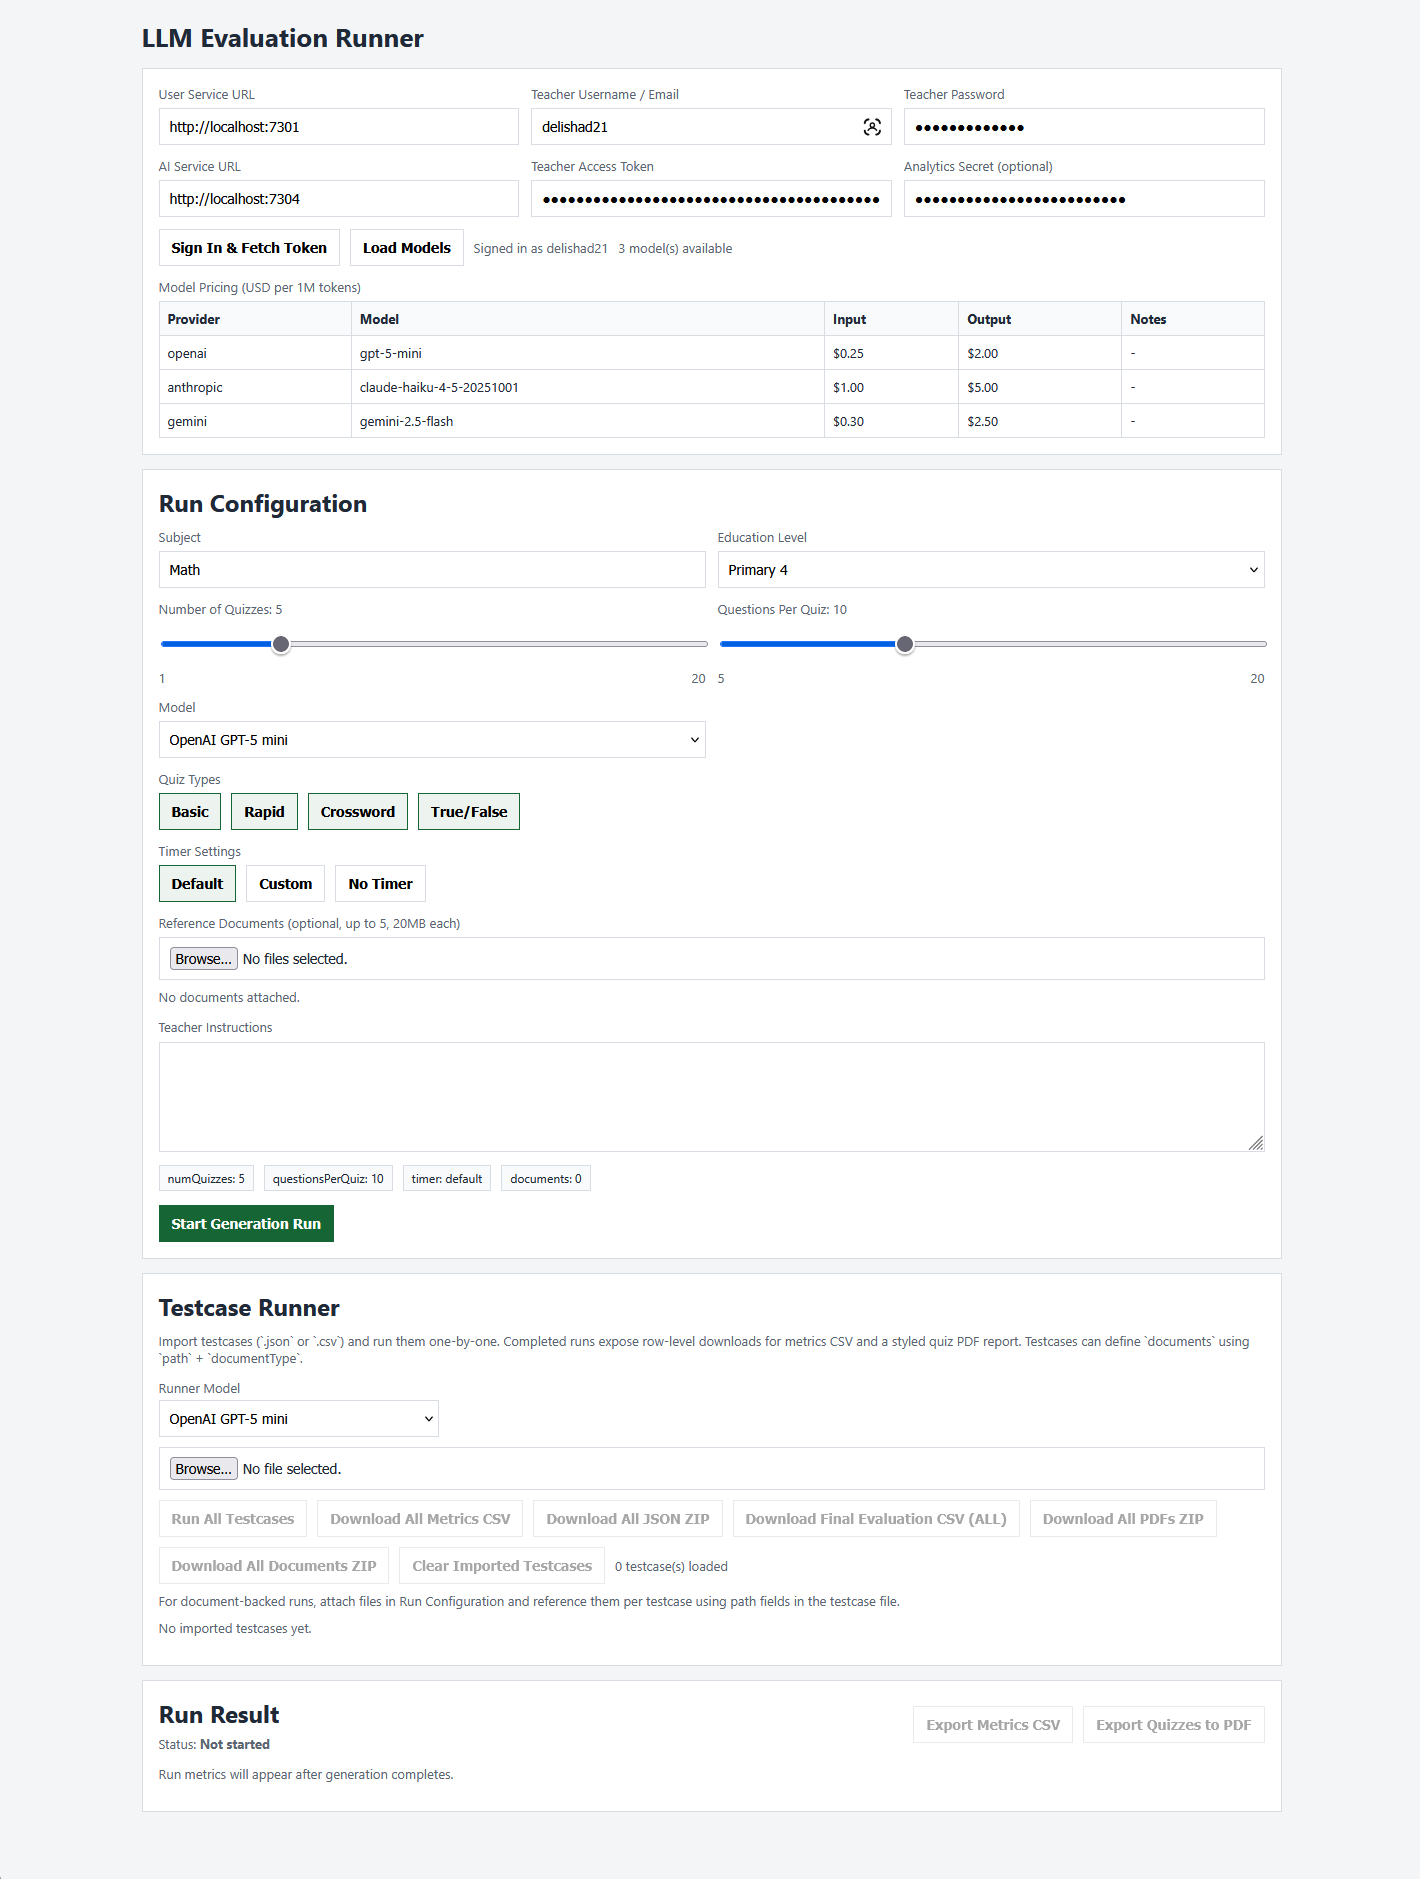
\includegraphics[width=0.82\textwidth]{assets/appendix-f/Figure_F_1_LLM_Eval_App_UI.png}
\end{center}


\section*{7. Deterministic Structural Validity Checks}


The LLM Eval App produces a structured JSON including the normalised generated quizzes and questions for each testcase, essentially the final version of the quiz outputted by the AI service.


Deterministic structural checks are run on these normalized quiz outputs exported per testcase to evaluate integrity and variety.


It is important to note that normalization already enforces many structural rules, such as minimum MC options and the presence of at least one correct answer, and will trigger retries if the output fails to meet those rules. The checks that are done here are to catch any escaped errors that slipped through normalization and still ended up in the final quiz structure. These escaped errors are errors that are not severe enough to trigger rejection during normalization, but they still remain as good indicators of the model's quality in generated quizzes.


From the responses generated by the models, a set of deterministic structural validity checks were applied to assess whether the generated content met the required format and structure for quiz content in the platform. These checks included the following:


\begin{enumerate}
\item \texttt{run\_quiz\_count\_mismatch}, which checks whether the generation run returned the expected total number of quizzes.
\item \texttt{quiz\_question\_count\_mismatch}, which checks whether each generated quiz contains the expected number of questions or entries.
\item \texttt{mc\_option\_count\_invalid}, which checks whether a multiple-choice item includes a sufficient number of answer options.
\item \texttt{mc\_correct\_count\_invalid}, which checks whether a multiple-choice item includes at least one correct answer.
\item \texttt{open\_missing\_answers}, which checks whether an open-ended item contains a valid answer structure.
\item \texttt{open\_exact\_missing\_text}, which checks whether an exact-match open-ended answer includes the required answer text.
\item \texttt{open\_keywords\_invalid}, which checks whether a keyword-based open-ended answer contains a valid keyword list and threshold.
\item \texttt{open\_list\_invalid}, which checks whether a list-based open-ended answer contains a valid list of items and a valid minimum-correct threshold.
\item \texttt{context\_missing\_text}, which checks whether a context item includes the passage or prompt text required for linked questions.
\item \texttt{crossword\_grid\_missing}, which checks whether a crossword quiz includes a valid crossword grid.
\item \texttt{crossword\_entry\_invalid}, which checks whether each crossword entry includes both a valid clue and a valid answer.
\end{enumerate}

The results of these checks were used to calculate the escape score for each generated quiz, which represents the percentage of checks that were passed successfully. This provides a quantitative measure of the structural validity of the generated content, which is a key aspect of generation quality for this platform.


For scoring, only these checks are included in the escaped-error denominator. Each applicable rule contributes one check to the total checks performed, and each failed rule increments the escaped error count by 1. A single item can fail multiple rules, and each failure is counted separately. The escaped error rate is calculated as \texttt{escaped\_error\_count / checks\_performed * 100}, and the escape score is calculated as \texttt{100 - escaped\_error\_rate}.


Following that, the generated content was evaluated for variety using


\begin{enumerate}
\item Unique stem ratio
\item Distinctness (1 minus average Jaccard similarity between generated questions)
\item Intent bucket coverage, which checks whether the generated questions cover a diverse range of question intents (e.g. recall, application, analysis) based on a predefined set of vocabulary.
\end{enumerate}

These checks are combined into a variety score, using the weighted formula \texttt{0.45 * unique\_stem\_ratio + 0.35 * distinctness + 0.20 * intent\_coverage}.


For this calculation, the script first extracts prompts as follows:


\begin{itemize}
\item for crossword quizzes, each clue is treated as a prompt
\item for other quiz types, each question text is treated as a prompt
\item context items are excluded from this calculation
\end{itemize}

Let \texttt{n} be the number of extracted prompts in a testcase run. If \texttt{n = 0}, then all variety metrics are set to \texttt{0}.


The prompts are then normalised before comparison:


\begin{itemize}
\item converted to lowercase
\item non-alphanumeric characters are replaced with spaces
\item repeated whitespace is collapsed
\item surrounding whitespace is trimmed
\end{itemize}

The exact metrics are calculated as follows:


\begin{enumerate}
\item \textbf{Unique Stem Ratio}: This measures how many prompts remain unique after normalisation.
\end{enumerate}

\begin{itemize}
\item \texttt{unique stem ratio = number of unique normalized prompts / n}
\item \texttt{variety\_unique\_stem\_ratio\_pct = unique stem ratio * 100}
\end{itemize}

\begin{enumerate}
\item \textbf{Distinctness}: This measures how different the prompts are from one another after tokenisation and stopword removal. \\ For each prompt:
\end{enumerate}

\begin{itemize}
\item the prompt is tokenised after normalisation
\item common stopwords are removed
\item Jaccard similarity is calculated against every other prompt \\ Jaccard similarity is:
\item \texttt{Jaccard(A, B) = |A ∩ B| / |A ∪ B|} \\ For each prompt \texttt{i}, the highest similarity to any other prompt is taken:
\item \texttt{max\_sim\_i = max(Jaccard(prompt\_i, prompt\_j)) for all j != i} \\ Then those maximum similarities are averaged:
\item \texttt{average maximum similarity = sum(max\_sim\_i) / n} \\ Distinctness is then:
\item \texttt{distinctness = 1 - average maximum similarity}
\item \texttt{variety\_distinctness\_pct = distinctness * 100}
\end{itemize}

\begin{enumerate}
\item \textbf{Intent Coverage}: This measures whether the prompts span a broader range of prompt intents. \\ Each prompt is assigned to one of six deterministic intent buckets:
\end{enumerate}

\begin{itemize}
\item \texttt{reasoning}
\item \texttt{compare}
\item \texttt{procedure}
\item \texttt{listing}
\item \texttt{recall}
\item \texttt{application} \\ The script classifies each prompt by matching keywords associated with each intent bucket. If none of the earlier buckets match, the prompt is classified as \texttt{application}.
\item \texttt{intent coverage = number of unique intent buckets present / 6}
\item \texttt{variety\_intent\_coverage\_pct = intent coverage * 100}
\end{itemize}

The final variety score is then exported as:


\begin{itemize}
\item \texttt{variety\_score\_pct = (0.45 * unique stem ratio + 0.35 * distinctness + 0.20 * intent coverage) * 100}
\end{itemize}

The final exported percentage values are rounded to 4 decimal places.


\section*{8. Reliability and Performance Metrics}


In addition to the quality checks described above, this evaluation also measures the reliability and performance of the models. The purpose of this is to assess how consistently each of the models could generate usable outputs that can be processed by the platform, as well as how long the generation process takes.


These metrics came from the LLM eval app's run exports.


The following metrics were measured.


\begin{enumerate}
\item \textbf{Completion Rate}: This measures each job success. If the job produced a valid output, it counts as a success, even if some outputs were invalid and retried. The completion rate is calculated as \texttt{successful / expected * 100}.
\item \textbf{Retry Count}: This captures robustness of the LLM in producing valid outputs without needing retries. High retry counts indicate instability of the model for the given generation task.
\item \textbf{Attempt Count}: This measures the total number of generation attempts made for each test case. This metric is mainly used to interpret and normalize the retry count.
\item \textbf{Total Latency}: This is cumulative latency across all LLM calls in the run, including the planning call, every generation call, and any retry calls.
\end{enumerate}

Other fields were also recorded for analysis, though they were not included in the final automated score:


\begin{enumerate}
\item \textbf{Token Usage}: Planning tokens, generation tokens, and overall total tokens were recorded for reporting and cross-model efficiency comparison. Most LLM provider pages indicate that extracted token usage is still an estimate and may not match exact billing cost, but from testing and the costs incurred on actual usage, these values were found to be relatively accurate.
\item \textbf{Estimated Cost}: Estimated cost was computed in the evaluator app via a model pricing table from token usage. These prices were hard coded into the evaluator configuration based on public pricing tables for each model, and were accurate as of March 2026, but would not reflect future price changes.
\end{enumerate}

Using the metrics above, three different reliability and performance scores are calculated:


\begin{enumerate}
\item \textbf{Completion Score}: \texttt{completion\_score\_100 = 100 * (completion\_rate\_pct / 100)\textasciicircum{}2}. This score is designed to heavily reward higher completion rates, as generation completion is a critical aspect of reliability for this platform. As such, the completion rate is squared in the formula to more heavily penalise lower completion rates.
\item \textbf{Retry Score}: \texttt{retry\_score\_100 = 100 * max(0, 1 - retry\_count / max(1, attempt\_count))\textasciicircum{}3}. This score is designed to reward lower retry counts, as a high number of retries can indicate that the model is generating content that often fails the validity checks, which increases latency and cost, and is generally indicative of the model being less capable of generating usable content. The retry count is normalised by the total attempt count to account for cases where the model may have a low completion rate, and the score is cubed to more heavily penalise higher retry rates.
\item \textbf{Latency Score}: Latency score is calculated using the following bands of response times:
\end{enumerate}

{
\fontsize{10}{12}\selectfont
\setlength{\tabcolsep}{4pt}
\renewcommand{\arraystretch}{1.15}
\begin{xltabular}{\textwidth}{|>{\raggedright\arraybackslash}p{4.2cm}|>{\raggedright\arraybackslash}X|}
\hline
\textbf{Total LLM latency per run} & \textbf{\texttt{latency\_score}} \\ \hline
\endhead
\texttt{<= 60,000 ms} & 80 \\ \hline
\texttt{60,001 - 120,000 ms} & 55 \\ \hline
\texttt{120,001 - 180,000 ms} & 40 \\ \hline
\texttt{180,001 - 240,000 ms} & 30 \\ \hline
\texttt{240,001 - 300,000 ms} & 20 \\ \hline
\texttt{300,001 - 420,000 ms} & 10 \\ \hline
\texttt{> 420,000 ms} & 0 \\ \hline
\end{xltabular}
}


To calculate the overall reliability and performance score for each model, the three scores above are combined using the following weighted formula:


\texttt{reliability\_score\_100 = 0.45*completion\_score\_100 + 0.35*retry\_score\_100 + 0.20*latency\_score}


This formula weighs each component according to its importance for the platform, with completion rate being the most heavily weighted, followed by retry count, and then latency. This provides a comprehensive measure of the reliability and performance of each model in generating usable quiz content for the platform.


\section*{9. Structural Validity, Variety, and Reliability Results}


The measured results for structural validity, variety, and reliability are shown below.


{
\fontsize{10}{12}\selectfont
\setlength{\tabcolsep}{4pt}
\renewcommand{\arraystretch}{1.15}
\begin{xltabular}{\textwidth}{|>{\raggedright\arraybackslash}X|>{\raggedright\arraybackslash}X|>{\raggedright\arraybackslash}X|>{\raggedright\arraybackslash}X|>{\raggedright\arraybackslash}X|>{\raggedright\arraybackslash}X|}
\hline
\textbf{Model} & \textbf{Escaped Error Rate} & \textbf{Avg Escape Score} & \textbf{Runs with Escaped Errors} & \textbf{Avg Variety Score} & \textbf{Mean Reliability Score} \\ \hline
\endhead
Claude Haiku 4.5 & 0.0830\% & 99.9013 & 2/24 & 82.3380 & 86.7756 \\ \hline
GPT-5 mini & 0.3633\% & 99.6340 & 8/24 & 83.8721 & 82.5731 \\ \hline
Gemini 2.5 Flash & 0.0000\% & 100.0000 & 0/24 & 82.2321 & 88.0129 \\ \hline
\end{xltabular}
}


The following are the measured results for completion rate, retry count, attempt count, total latency, and reliability score.


{
\fontsize{10}{12}\selectfont
\setlength{\tabcolsep}{4pt}
\renewcommand{\arraystretch}{1.15}
\begin{xltabular}{\textwidth}{|>{\raggedright\arraybackslash}X|>{\raggedright\arraybackslash}X|>{\raggedright\arraybackslash}X|>{\raggedright\arraybackslash}X|>{\raggedright\arraybackslash}X|}
\hline
\textbf{Model} & \textbf{Mean Completion Rate} & \textbf{Mean Retry Count} & \textbf{Mean Attempt Count} & \textbf{Mean Total LLM Latency} \\ \hline
\endhead
Claude Haiku 4.5 & 99.17\% & 0.75 & 5.71 & 59,154 ms \\ \hline
GPT-5 mini & 100.00\% & 0.08 & 5.08 & 296,047 ms \\ \hline
Gemini 2.5 Flash & 100.00\% & 0.25 & 5.25 & 97,507 ms \\ \hline
\end{xltabular}
}


\section*{10. Token Usage and Cost Analysis}


The following table shows the average token usage and cost estimates for all total runs.


These token and cost calculations were not factored into the final scores for the models, as the main focus of this evaluation was on the quality and reliability of the generated content. However, cost is still an important consideration for the platform, especially as it scales, so these estimates were still kept track of and are provided here for reference.


{
\fontsize{10}{12}\selectfont
\setlength{\tabcolsep}{4pt}
\renewcommand{\arraystretch}{1.15}
\begin{xltabular}{\textwidth}{|>{\raggedright\arraybackslash}X|>{\raggedright\arraybackslash}X|>{\raggedright\arraybackslash}X|>{\raggedright\arraybackslash}X|}
\hline
\textbf{Model} & \textbf{Mean Overall Tokens / Run} & \textbf{Mean Estimated Cost / Run (USD)} & \textbf{Total Estimated Cost for 24 Runs (USD)} \\ \hline
\endhead
Claude Haiku 4.5 & 17,871 & 0.058409 & 1.401820 \\ \hline
GPT-5 mini & 25,677 & 0.039730 & 0.953512 \\ \hline
Gemini 2.5 Flash & 27,905 & 0.028908 & 0.693788 \\ \hline
\end{xltabular}
}


\section*{11. Comparative Results Across Models}


To summarise the comparative results across the three models, a final overall score was calculated for each model by combining the quality metrics (structural validity and variety) with the reliability score, using the following weighted formula:


\texttt{overall\_run\_score = 0.70*reliability + 0.20*integrity + 0.10*variety}


This formula places priority on the reliability metrics, as in the context of this platform, having a model that cannot complete runs consistently, has a high retry rate, or has a high latency can significantly impact the user experience more so than small differences in the structural validity or variety of the generated content.


Structural validity and variety are still important, but they are weighted lower in the overall score as these two mainly serve as narrow quality measures. Deterministic measures can only realistically capture certain aspects of generation quality, and there are many other important dimensions of quality such as the educational relevance, the appropriateness of the language used, and the creativity of the generated content that are not captured by these metrics. Assessing meaningful variety in generated content is also a lot more intricate, and would likely require human evaluation from subject matter experts to provide a more accurate assessment. As such, these two metrics are weighted lower in the overall score, serving more as supportive measures to the reliability score.


Using this automated scoring formula, the following model-level scores were obtained by averaging the run-level automated scores across the 24 testcases for each model.


{
\fontsize{10}{12}\selectfont
\setlength{\tabcolsep}{4pt}
\renewcommand{\arraystretch}{1.15}
\begin{xltabular}{\textwidth}{|>{\raggedright\arraybackslash}p{4.2cm}|>{\raggedright\arraybackslash}X|}
\hline
\textbf{Model} & \textbf{Overall Automated Score (/100)} \\ \hline
\endhead
Gemini 2.5 Flash & 89.8322 \\ \hline
Claude Haiku 4.5 & 88.9570 \\ \hline
GPT-5 mini & 86.1152 \\ \hline
\end{xltabular}
}


These results indicate that Gemini 2.5 Flash achieved the highest overall automated score in this evaluation cycle, followed closely by Claude Haiku 4.5, while GPT-5 mini ranked third on the same scoring basis.


\section*{12. Planned Human Evaluation of Generation Quality}


As briefly touched upon in the earlier section, deterministic assessments of generation quality can only go so far in capturing the true quality of the generated content, especially in an educational context where the relevance, appropriateness, and creativity of the content are crucial factors that are not easily quantifiable. It is also worth noting that there was some level of human evaluation achieved in the secondary user testing, as teachers were asked to evaluate the quality of the generated content. Most responses indicated that there was much to improve in the quality of the generated content, but the few responses are insufficient to provide a definitive assessment of the improvements needed in the generated content.


As such, plans for a follow-up human evaluation of the generated content were drafted up, simply lacking the resources to be executed in this initial phase of AI generated evaluation. The human evaluation will involve subject matter experts in education who will review samples of the generated quizzes, obtained from the same test cases used in the automated evaluation.


Experts will evaluate the quizzes across four dimensions that attempt to capture the key aspects of generation quality that are relevant for the platform:


\begin{enumerate}
\item Alignment to prompt
\item Alignment to syllabus or curriculum intent
\item Question correctness
\item Question variety
\end{enumerate}

The following is a proposed rubric for the human evaluation.


{
\fontsize{10}{12}\selectfont
\setlength{\tabcolsep}{4pt}
\renewcommand{\arraystretch}{1.15}
\begin{xltabular}{\textwidth}{|>{\raggedright\arraybackslash}X|>{\raggedright\arraybackslash}X|>{\raggedright\arraybackslash}X|>{\raggedright\arraybackslash}X|>{\raggedright\arraybackslash}X|>{\raggedright\arraybackslash}X|}
\hline
\textbf{Dimension} & \textbf{1 (Poor)} & \textbf{2 (Weak)} & \textbf{3 (Adequate)} & \textbf{4 (Good)} & \textbf{5 (Excellent)} \\ \hline
\endhead
Alignment to prompt & Largely ignores the teacher request, with incorrect focus or level. & Partly follows the request, but with major drift in focus or level. & Mostly follows the request, with some drift or inconsistency. & Clearly follows the request, with only minor issues. & Fully follows the request, with precise focus and level throughout. \\ \hline
Alignment to syllabus/curriculum intent & Frequently below or above the expected primary level, or off-topic. & Contains multiple curriculum-level mismatches. & Generally suitable in level and topic, but with uneven coverage. & Shows good level fit and topic relevance across most questions. & Demonstrates strong curriculum fit, level-appropriateness, and highly relevant coverage throughout. \\ \hline
Question correctness & Contains many incorrect, ambiguous, or invalid items or answer keys. & Contains several incorrect or ambiguous items. & Mostly correct, but with a few issues. & Correct and clear, with only rare minor issues. & Consistently correct, clear, and unambiguous. \\ \hline
Question variety & Very repetitive in stems and skill types. & Limited variety, with frequent repetition. & Moderate variety, with some repetition. & Good mix of skills, phrasing, and contexts. & Excellent variety in skills, phrasing, and contexts without losing focus. \\ \hline
\end{xltabular}
}


For aggregation, each rating will be converted to a 100 point scale


\begin{enumerate}
\item \texttt{prompt\_score = prompt\_rating * 20}
\item \texttt{curriculum\_score = curriculum\_rating * 20}
\item \texttt{correctness\_score = correctness\_rating * 20}
\item \texttt{variety\_score\_manual = variety\_rating * 20}
\end{enumerate}

The weighted manual score will then be calculated using the following formula.


\texttt{manual\_score = 0.25*prompt\_score + 0.25*curriculum\_score + 0.35*correctness\_score + 0.15*variety\_score}


This weighting gives the highest priority to correctness, as having incorrect or ambiguous questions can significantly undermine the educational value of the generated content. Alignment to the prompt and curriculum are also important, but they are weighted slightly lower as they can be somewhat more subjective and may have a bit more flexibility depending on the teacher's intent. Variety is still an important aspect of quality, but it is weighted lowest in this rubric as it is more of a nice-to-have feature rather than a critical requirement for the generated content.


The manual ratings can optionally be combined with the automated metrics to provide a more comprehensive overall score for the generated content, using a formula such as:


\texttt{overall\_run\_score\_with\_manual = 0.60*manual\_score + 0.40*overall\_run\_score}


This was defined as a future extension. The automated evaluation is the main completed method in this project phase.


\section*{13. Threats to Validity}


There are several limitations of this evaluation that should be acknowledged:


\begin{enumerate}
\item The automated evaluation was intentionally run without uploaded documents due to cost limitations. So the results that were obtained mainly reflect prompt-driven behaviour without any supplementary material. This may still be representative of the actual use case for the platform, as teachers may often use the AI generation features without uploading additional documents, but it does mean that the evaluation does not capture how well the models can leverage uploaded materials to enhance the quality and relevance of the generated content.
\item Manual evaluation is still needed to capture important dimensions of quality that are not easily quantifiable, such as the educational relevance and appropriateness of the generated content. The planned human evaluation will help to address this limitation, but it is still a limitation of the current evaluation results.
\item Deterministic structural checks are structural and integrity-oriented, not a full pedagogical evaluation.
\item Deterministic variety remains a heuristic proxy, not a replacement for expert judgment.
\item Without manual review, curriculum depth, wording quality, and pedagogical suitability are only partially captured.
\end{enumerate}
